\section{General}
Walls in the building construction industry are defined as structural elements that generally form an enclosed area. The walls form an integral entity of a construction unit in any sector in the construction industry (residential, commercial, industrial). Different types of walls are used and the type of wall varies with respect to the utility in the building. For instance, in the residential sector, the walls used are made of wood, solid masonry and cavity masonry etc. Apart from these conventional methods of wall construction the usage of light gauge steel frames (LSF) in walls has been found to be a better alternative in drywall systems due to the many advantages including speedy construction . 

The use of LSF walls is rapidly increasing in the residential and commercial sectors of the construction industry. In the LSF walls, cold-formed steel channel sections are generally used as a skeleton for the wall panels which are usually sandwiched between plasterboards. The plasterboards are generally a combination of gypsum inner core lined with heavy duty paper. The LSF walls can also include cavity or external insulation and can be load bearing or non-load bearing. Many factors influence the structural and thermal performance of these LSF walls exposed to fire conditions. Apart from the structural loads such as dead/live loads, seismic and wind loads acting on the building, thermal loads due to the outbreak of fire in a building can also be a vital cause for the failure of the walls.  The structural performance of LSF walls is generally governed by the behaviour of cold-formed steel studs under the applied loads at elevated temperatures. Thermal performance of LSF walls is mainly governed by the plasterboards and steel studs as both these entities transfer heat. The geometric configuration of the studs within LSF walls significantly governs the thermal performance of LSF walls and thus also the structural performance of load bearing LSF walls. But to date majority of research has been carried out only for walls with single row of stud. Few researchers have attempted to investigate the fire behaviour double stud walls but had many shortcomings in their research. For instance, \citet{Kodur2006} experimentally investigated the thermal performance of LSF walls with double rows of typical stud section. Numerical validation for the same was not carried out. Likewise, it is inferred that the use of typical LSF wall system with lipped channel sections for heights exceeding 3 m is not preferred. However, this situation can occur in places such as cinema theatres, hospitals, schools, partitions between houses in an apartment and between town houses.

In the above-mentioned places the acoustic insulation is also a major concern, and the performance of the single stud walls even with cavity insulation is not sufficient. The weighted sound residual index $R_w$ of LSF wall varies with respect to its configuration. $R_w$ value of 60 is rated to be an excellent insulation against sound from external sources. Therefore, to achieve the required $R_w$ index, complex LSF wall systems are widely used. The use of LSF walls with multi-stud wall systems will be beneficial in mid-rise buildings built with cold-formed steel sections as shown in Figures \ref{fig:midrise}~(a)~and~(b). Mid-rise buildings are generally residential apartments, small commercial complexes where the effective height is not more than 25 m as per National Construction Code (NCC). To satisfy the sound insulation requirement between the partitions, walls with two rows of stud are used. Various components and properties of LSF wall systems are briefly described next. However, this research is focused on the double and staggered stud wall systems.
	 
\begin{figure}[htbp]
	\centering	
		\begin{tabular}{cc}
			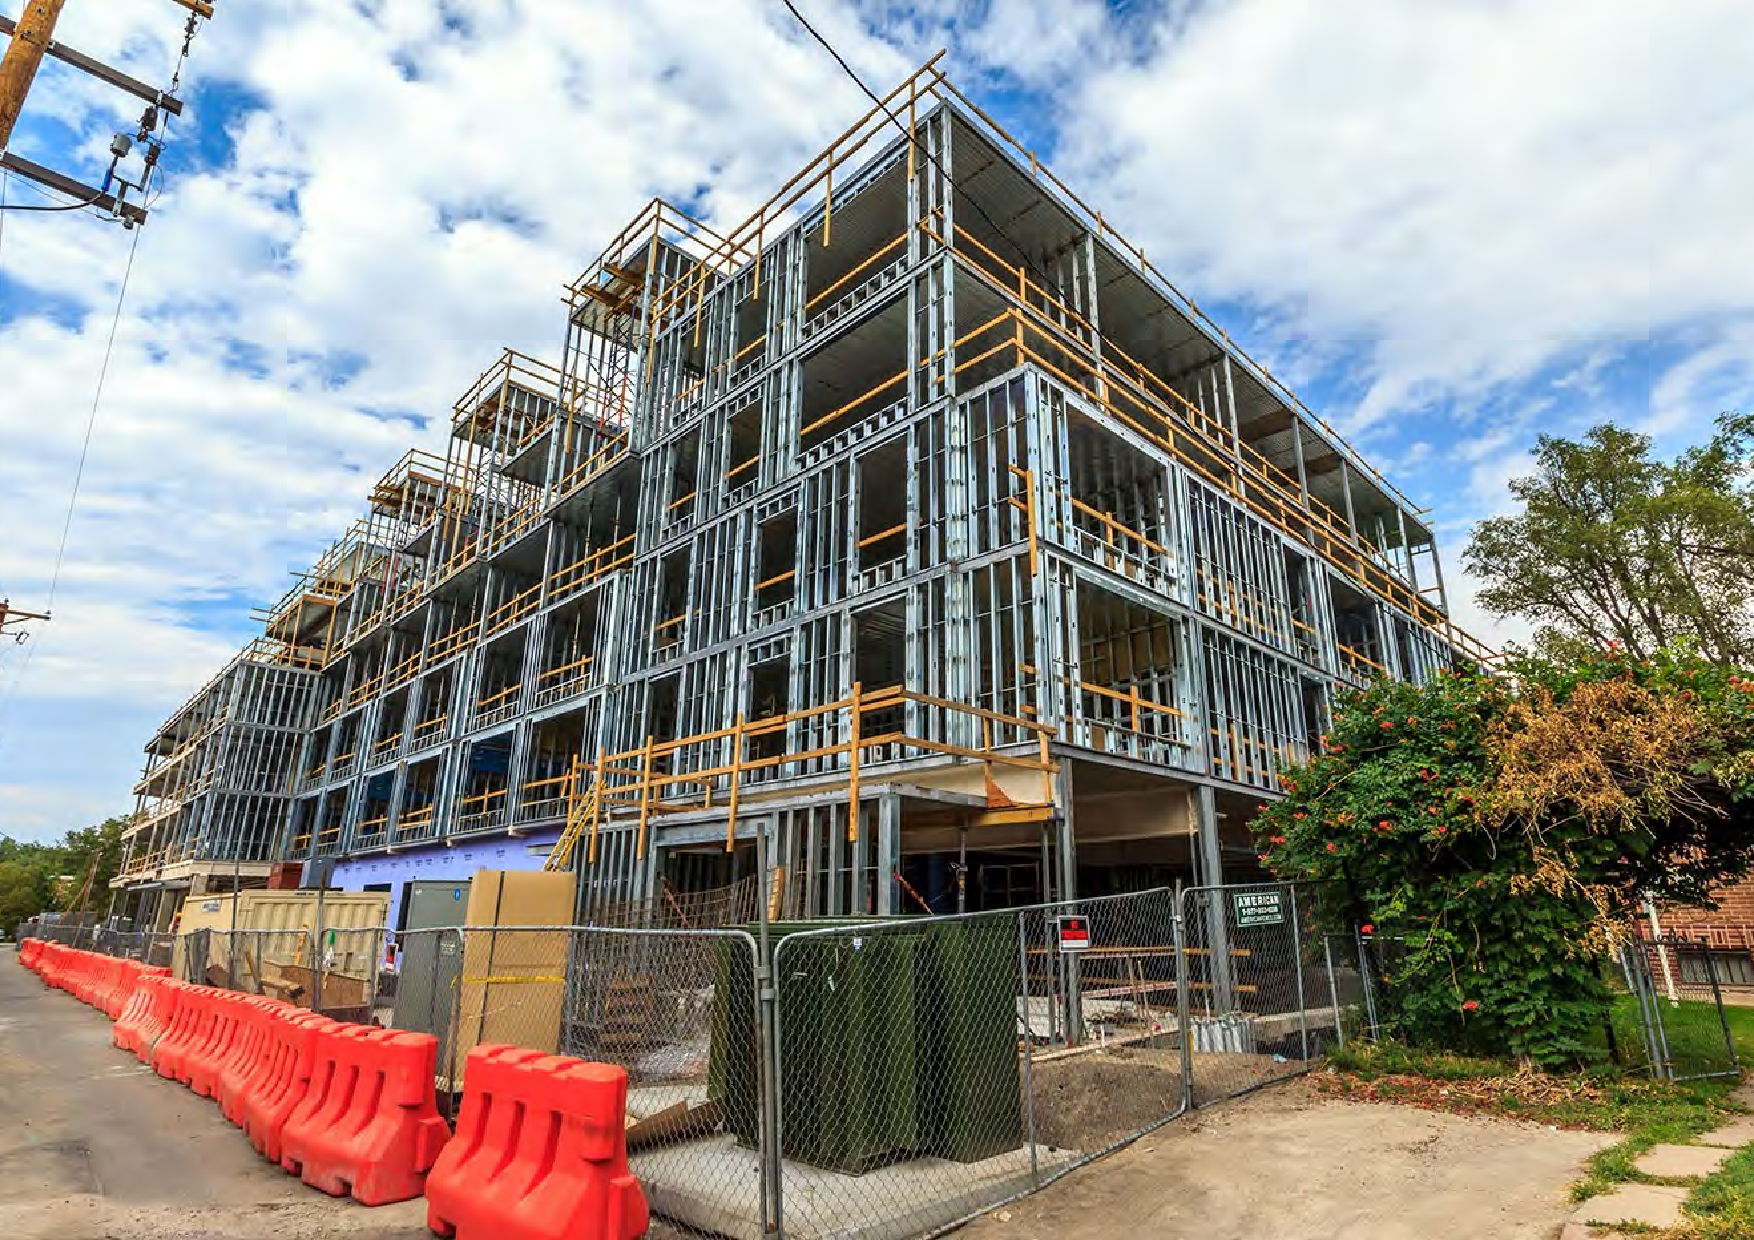
\includegraphics[width=7cm,height=5cm]{midrise1.pdf} &
			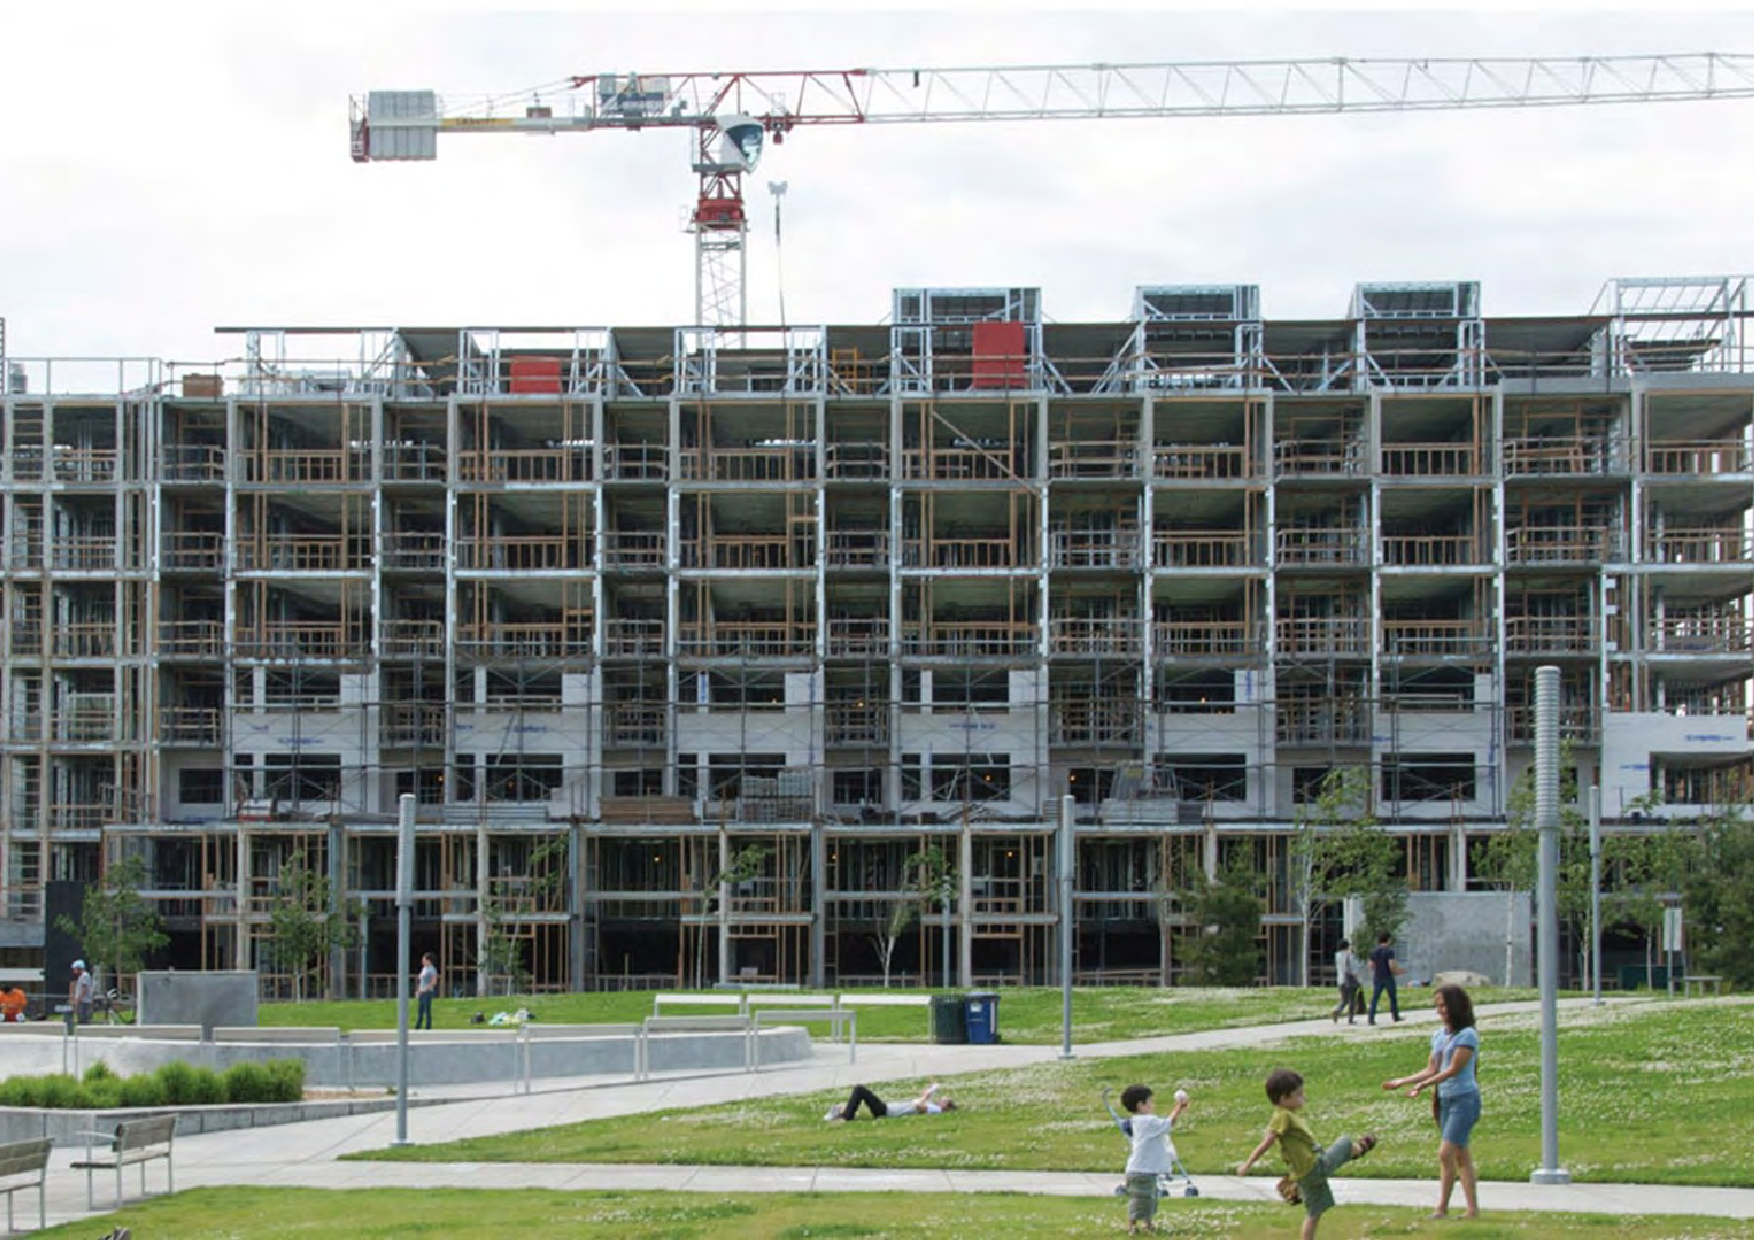
\includegraphics[width=7cm,height=5cm]{midrise2.pdf} \\
			(a) &
			(b) \\
		\end{tabular}
		\begin{scriptsize}
			Images extracted from (a) \url{https://starcash.co/steel-frame-building/astonishing-modular-products-prefabmarket/} (b) \url{https://ssfengineers.com/wp-content/uploads/2015/07/ballard-onthepark-b-copyright-bumgardner-architects-1920x1080.jpg}
			\end{scriptsize}	
		\caption{Mid-rise buildings with LSF wall system}
		\label{fig:midrise}
\end{figure}

\section{LSF Wall System}
\subsection{LSF Wall Components}

Light gauge steel frame / Lightweight steel frame wall systems are the latest advancements in modern wall construction. The main components of LSF wall systems include gypsum plasterboards, cold-formed steel sections (skeleton for the wall system), screws and other types of fasteners. The auxiliary components such as studs, tracks and noggings together form the skeleton of LSF wall system. The outer layer of the LSF wall system comprises of gypsum plasterboards. \Cref{fig:lsf_components} shows the components of a conventional LSF wall system based on a single row of studs in detail. The commonly used C-Section studs with double layers of plasterboard are shown in \Cref{fig:lsf_section}
\begin{figure}[htbp]
	\centering	
			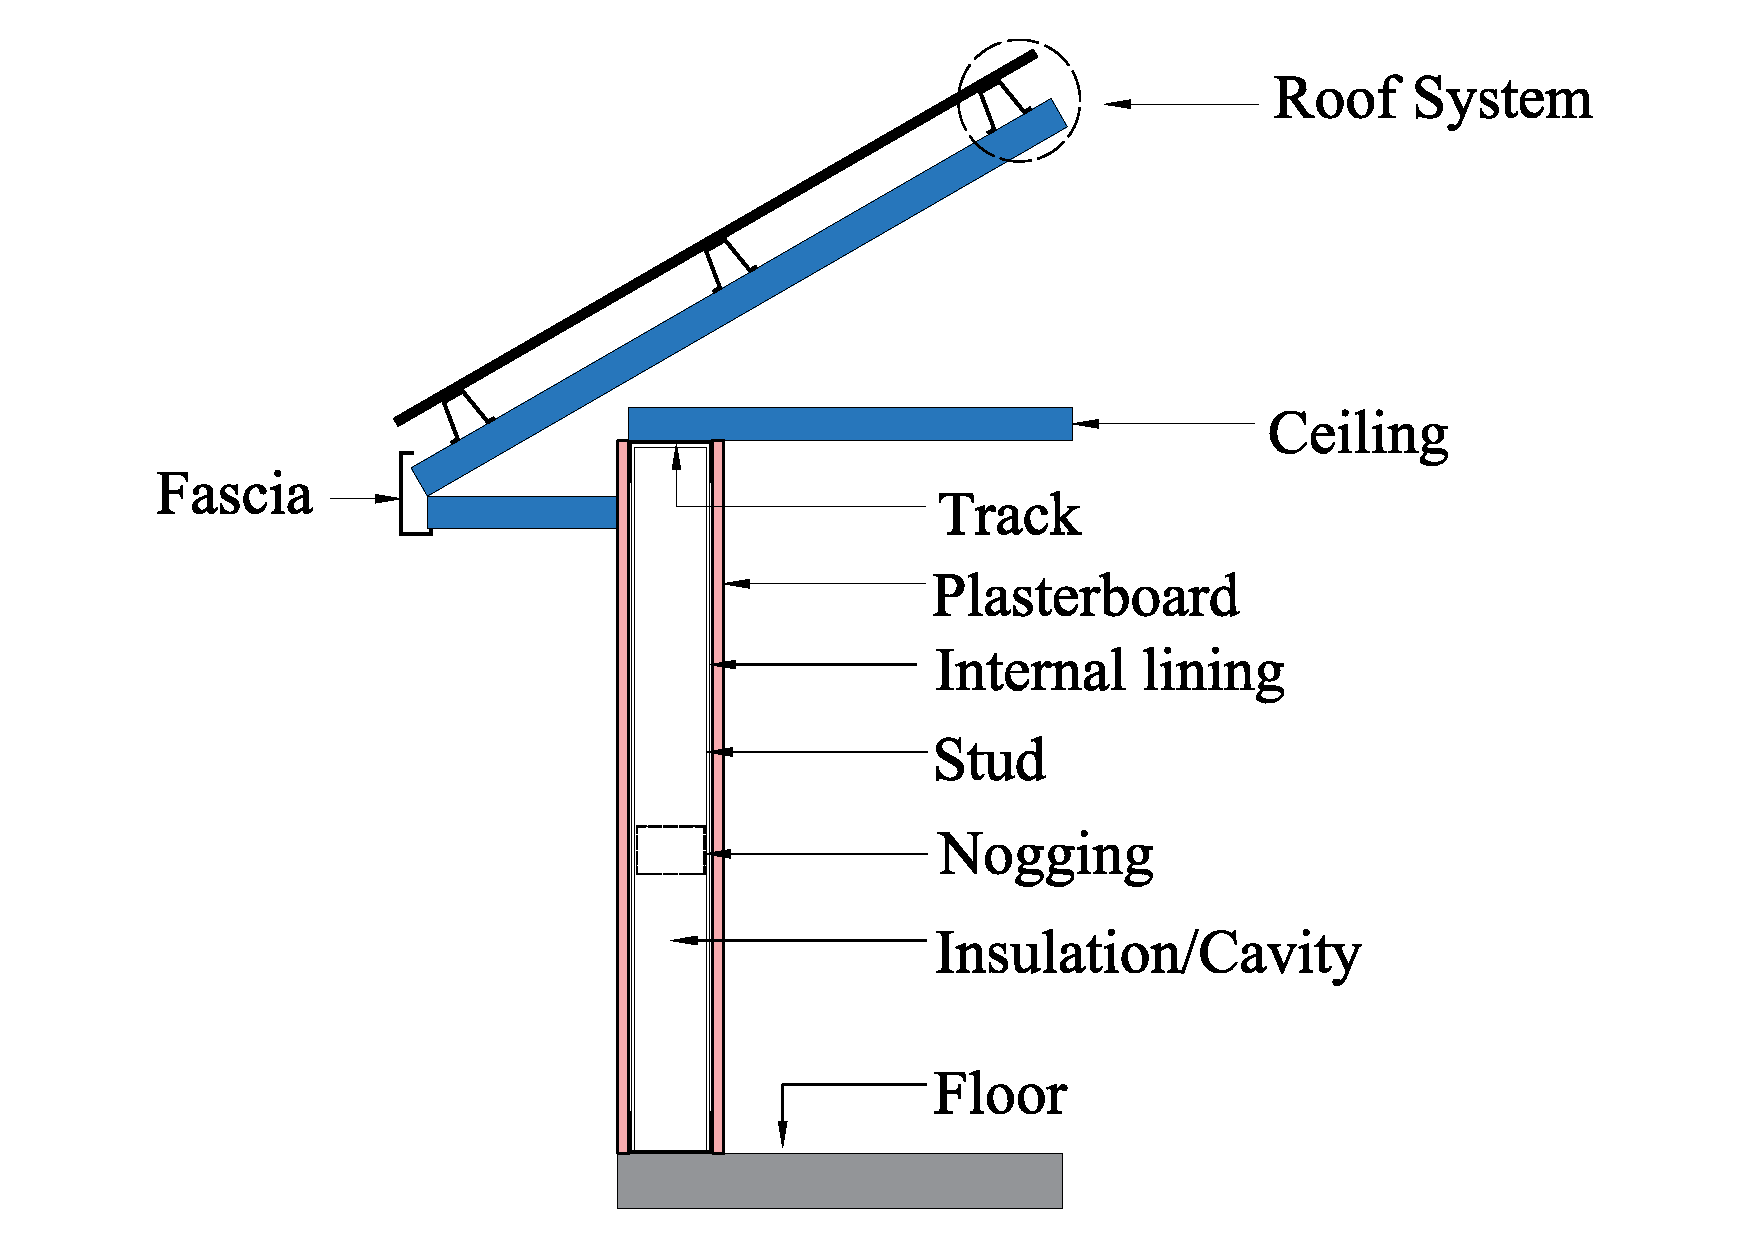
\includegraphics[width=9cm,height=7cm]{lsf_components.pdf}
				\caption{Components of LSF wall system}
		\label{fig:lsf_components}
\end{figure}
\begin{figure}[htbp]
	\centering	
		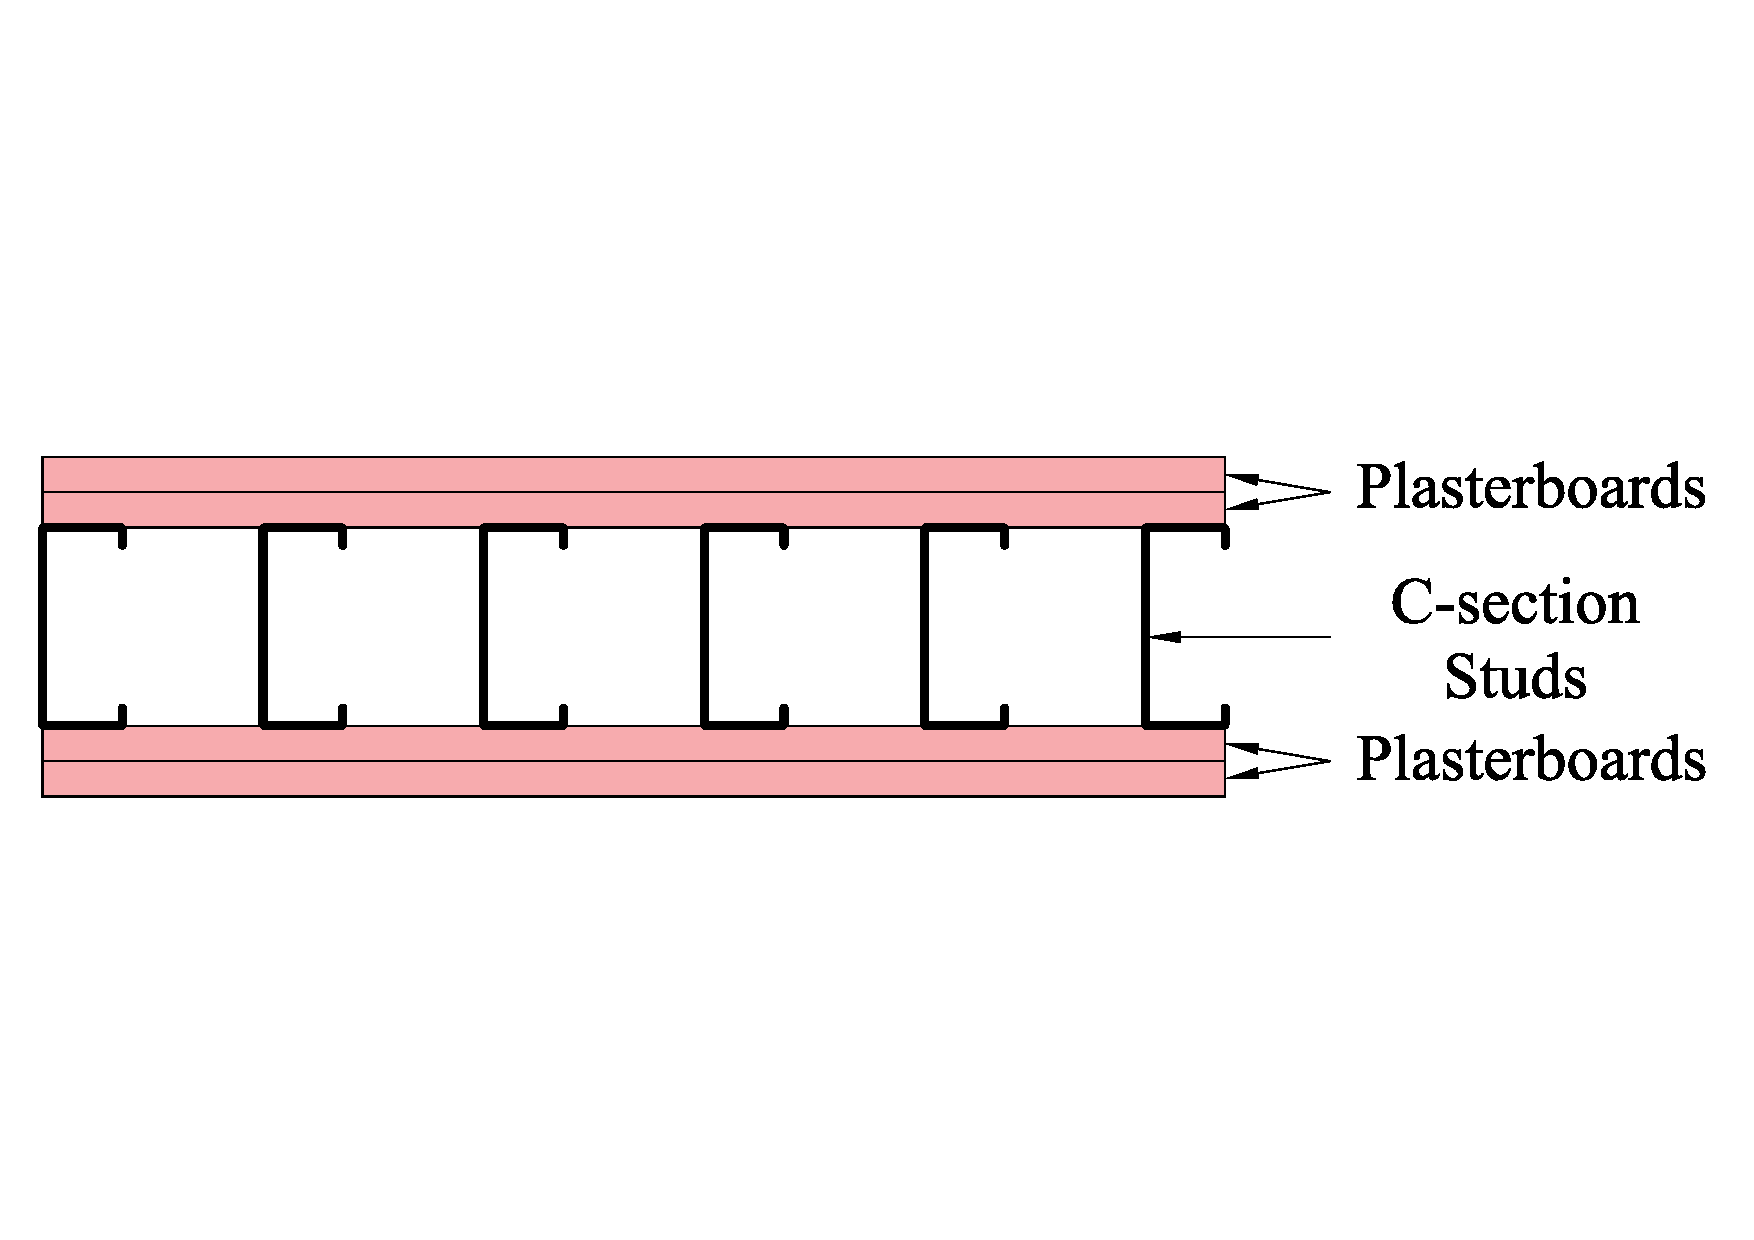
\includegraphics[width=10cm,height=2cm]{lsf_section.pdf}
		\caption{Plan view of LSF wall with Lipped C-Studs and double layers of plasterboard}
		\label{fig:lsf_section}
\end{figure}

In recent times, LSF wall, known as drywall, is an important constituent of modular building construction. Drywall also known as plasterboard are panel boards resembling plywoods and cardboards which are made of gypsum possessing the chemical name of Calcium sulphate dihydrate (CaSO4.2H2O). Plasterboards are manufactured by a process where the raw gypsum is dehydrated and then rehydrated to form calcium sulphate hemi hydrate. This is followed by mixing plaster with plasticizers and a foaming agent to achieve the necessary consistency. Ethelynediaminetetraacetic acid (EDTA) is used as a retardant in the manufacturing process to reduce the dew point, finally resulting in a pulp. This pulp is then sandwiched between two hard papers or fibre glass mats to form plasterboards. Some of the advantages of the plasterboard include ease of installation, thermal insulation, acoustic insulation and cost effectiveness.

Listed below are some of the advantages of LSF wall systems over conventional wall systems.

\begin{itemize}
\item Relatively low cost involved in the mass production of cold-formed steel sections.
\item Self-weight of the structure is less resulting in easier handling on site, minimizing the equipment handling cost.
\item Less time involved in constructing these walls in comparison with other wall systems.
\item Non-combustible in nature providing better fire resistance when compared to other wall systems as steel is the major component.
\item Better acoustic insulation as insulation layers can be customized within the wall panels as per end user requirement.
\item Eco-friendly construction as steel is the major component.
\item Resistance to termite attacks and weathering.
\end{itemize}

Even though the LSF wall systems possess many advantages, there are few areas in which the structural stability and strength of these wall systems can be compromised. One such area is the exposure of the LSF walls to elevated temperatures during fire exposure within or outside the building. Since steel is a good conductor of heat and the fact its mechanical properties deteriorate rapidly with increasing temperature, the cold-formed steel sections used within the LSF walls are vulnerable to both thermal and structural effects. Structural behaviour of LSF walls varies significantly at elevated temperatures when compared to ambient temperature conditions.

\subsection{Cold-formed Steel Sections}

Cold-formed steel sections are generally formed by cold pressing of thin steel sheets to the desired shape and size at ambient temperatures. Stamping and rolling methods are also employed for manufacturing some of the cold-formed steel sections. Cold-formed steel sections are generally designated as Channel/C-sections, Lipped channels, Nested Channels, I-sections, RHS (Rectangular Hollow Sections), CHS (Circular Hollow Sections), SHS (Square Hollow Sections), RHFCB (Riveted Hollow Flange Channel Beam) sections and Built-Up sections. Typical cold-formed steel sections are shown in \Cref{fig:typical_section}. Unlike the manufacturing process of hot-rolled steel sections, where the rolling of steel takes place at a very high temperature of 1700 \degree F (greater than the recrystallization temperature of steel), cold-formed steel sections are manufactured at room temperature.
\begin{figure}[htbp]
	\centering	
		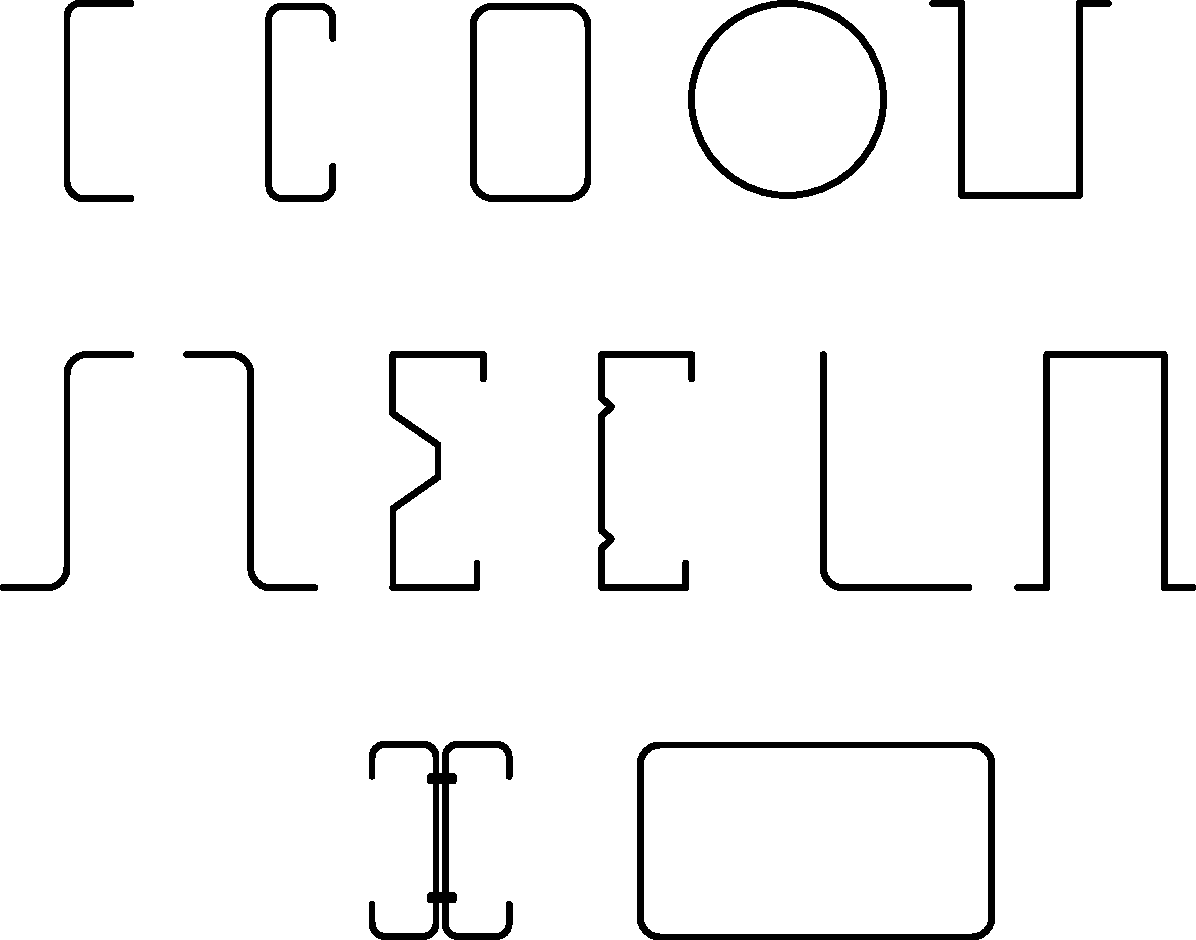
\includegraphics[width=7cm,height=5cm]{typical_sections.pdf}
		\caption{Typical Cold-Formed Steel Sections (CFS)}
		\label{fig:typical_section}
\end{figure}

Cold-formed steel can be termed as a derivative of hot-rolled steel as it is hot-rolled steel with further processing with a better surface finish than hot-rolled steel. The manufacturing process generally involves cold drawing, turning, grinding, polishing to get a smoother finish when compared to hot-rolled steel.

\subsection{Buckling Behaviour of Cold-Formed Steel Members}

As the name suggests, cold-formed steel sections are thin and their thickness varies from 0.55 mm to 8 mm. The thickness of cold-formed steel section is small in comparison with its width and thus local buckling of flanges/web will occur before section yielding. However, local buckling of the section does not imply that the section has reached its ultimate capacity. This phenomenon is referred to as post-buckling strength. Local buckling takes place at low compressive stresses as the width to thickness ratio is high in cold-formed steel sections.

The structural behaviour of cold-formed steel sections varies when compared to hot-rolled steel sections. This behaviour change is noticeable not only at ambient temperatures, but also at elevated temperatures. For instance, the plate and column slenderness ratios of cold-formed steel columns are higher than those of hot-rolled steel columns. This results in increased local and global buckling effects when compared to hot-rolled steel section columns. These effects can worsen at elevated temperatures. \Cref{fig:buckling_modes} shows the different types of buckling modes of a cold-formed steel column while \Cref{fig:buckling_plot} shows the corresponding buckling curve/plot. 
\begin{figure}[htbp]
	\centering	
		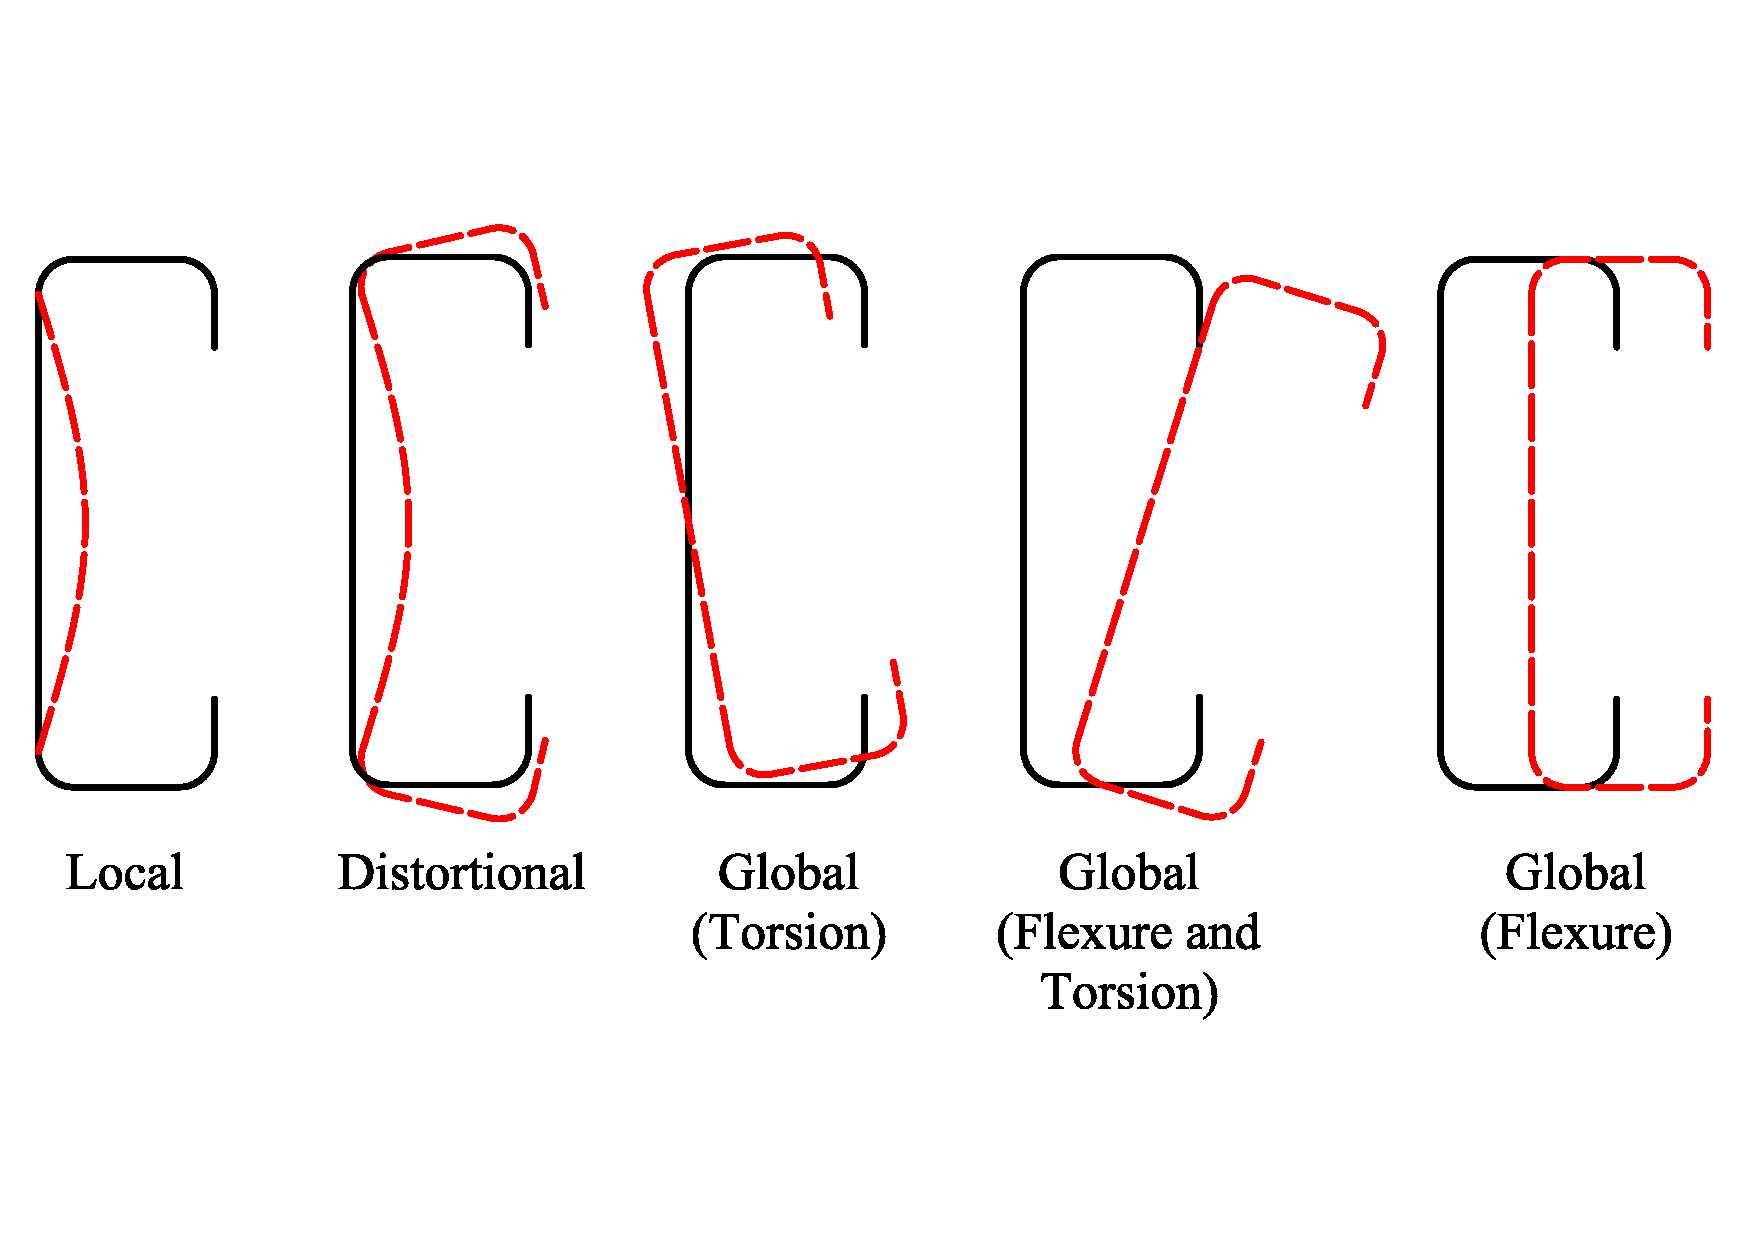
\includegraphics[width=8cm,height=3.5cm]{buckling_modes.pdf}
		\caption{Different buckling modes of a channel section column}
		\label{fig:buckling_modes}
\end{figure}
\begin{figure}[htbp]
	\centering	
		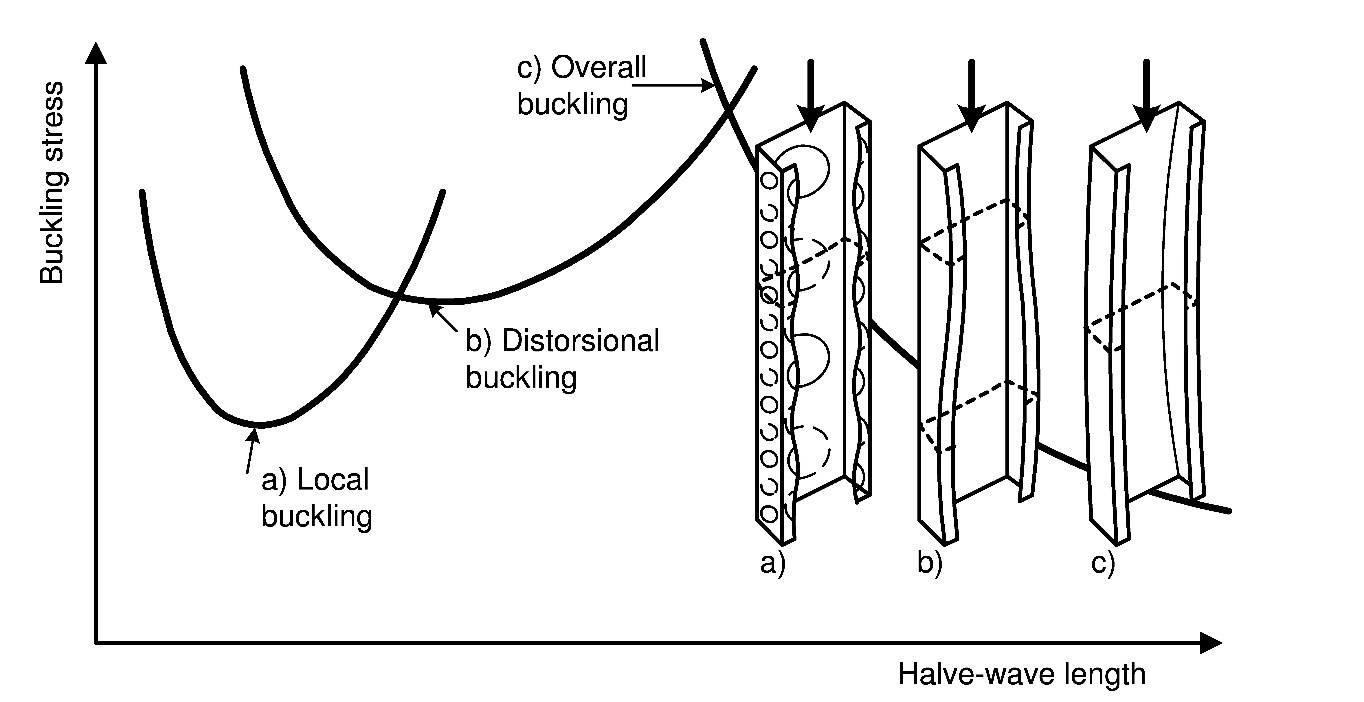
\includegraphics[width=8cm,height=4cm]{buckling_plot.jpg}
		\caption{Buckling plot from BS EN 1993-1-3 (2005a)}
		\label{fig:buckling_plot}
\end{figure}

\subsection{Design Guidelines}

The design standard pertaining to the structural design of cold-formed steel sections in Australia is AS/NZS 4600 (2014). Other design standards generally used in the cold-formed steel member design are AISI S100-12 ( 2007), AISI S202-15 and EN 1993-1-3:2006, which  provide the ambient temperature capacity equations for cold-formed steel members subjected to various actions such as compression, bending and their combinations. In the capacity calculations, the yield stress is taken as 0.2\% proof stress. When cold-formed steel members are exposed to fire conditions, specific design capacity equations are needed to predict the capacity deterioration due to fire. EN 1993-1-2 provides appropriate fire design rules, but they were mostly developed to suit hot-rolled steel members. Recent research by \citet{Ranawaka2009a}, \citet{Kankanamge2011} and \citet{Rokilan2019} have therefore focused on the behaviour and capacity determination of cold-formed steel members at elevated temperatures.

\subsection{Fire and Structural Performance of LSF walls}

Fire resistance level is used in the construction industry to determine the resistance to failure offered by structural components of a building in fire. This grading is designated in minutes under the following three criteria by NCC (2016).

\begin{itemize}
\item Structural adequacy - the ability to maintain adequate stability in fire.
\item Integrity - the ability to resist the passage of wall flames and fumes from the fire-exposed face of the wall to the unexposed face. 
\item Insulation - the ability to maintain a temperature on the surface of the unexposed face of the system to the limits specified as in AS/NZS 1530.4:2014 (SA, 2014).
\end{itemize}

The limiting values for the structural adequacy, integrity and insulation are specified in  NCC for various structural systems. The fire resistance level of an LSF wall is generally given in minutes (or hours) for each of the three criteria above.

Fire resistance of LSF walls is dependant on the thermal properties of the materials used in the wall system such as thermal conductivity, specific heat and relative density. \citet{Keerthan2012} investigated the thermal properties of gypsum plasterboards under standard fire conditions and provided a set of the thermal properties for use in the numerical models for validation purposes. The proposed thermal properties were also compared with the experimental fire test results of plasterboards and were observed to have good correlation. Cold-formed steel sections are often point symmetric, mono symmetric or non-symmetric, i.e. not doubly symmetric as shown in \Cref{fig:symmetry}. 
\begin{figure}[!htbp]
	\centering
		\begin{tabular}{cc}
			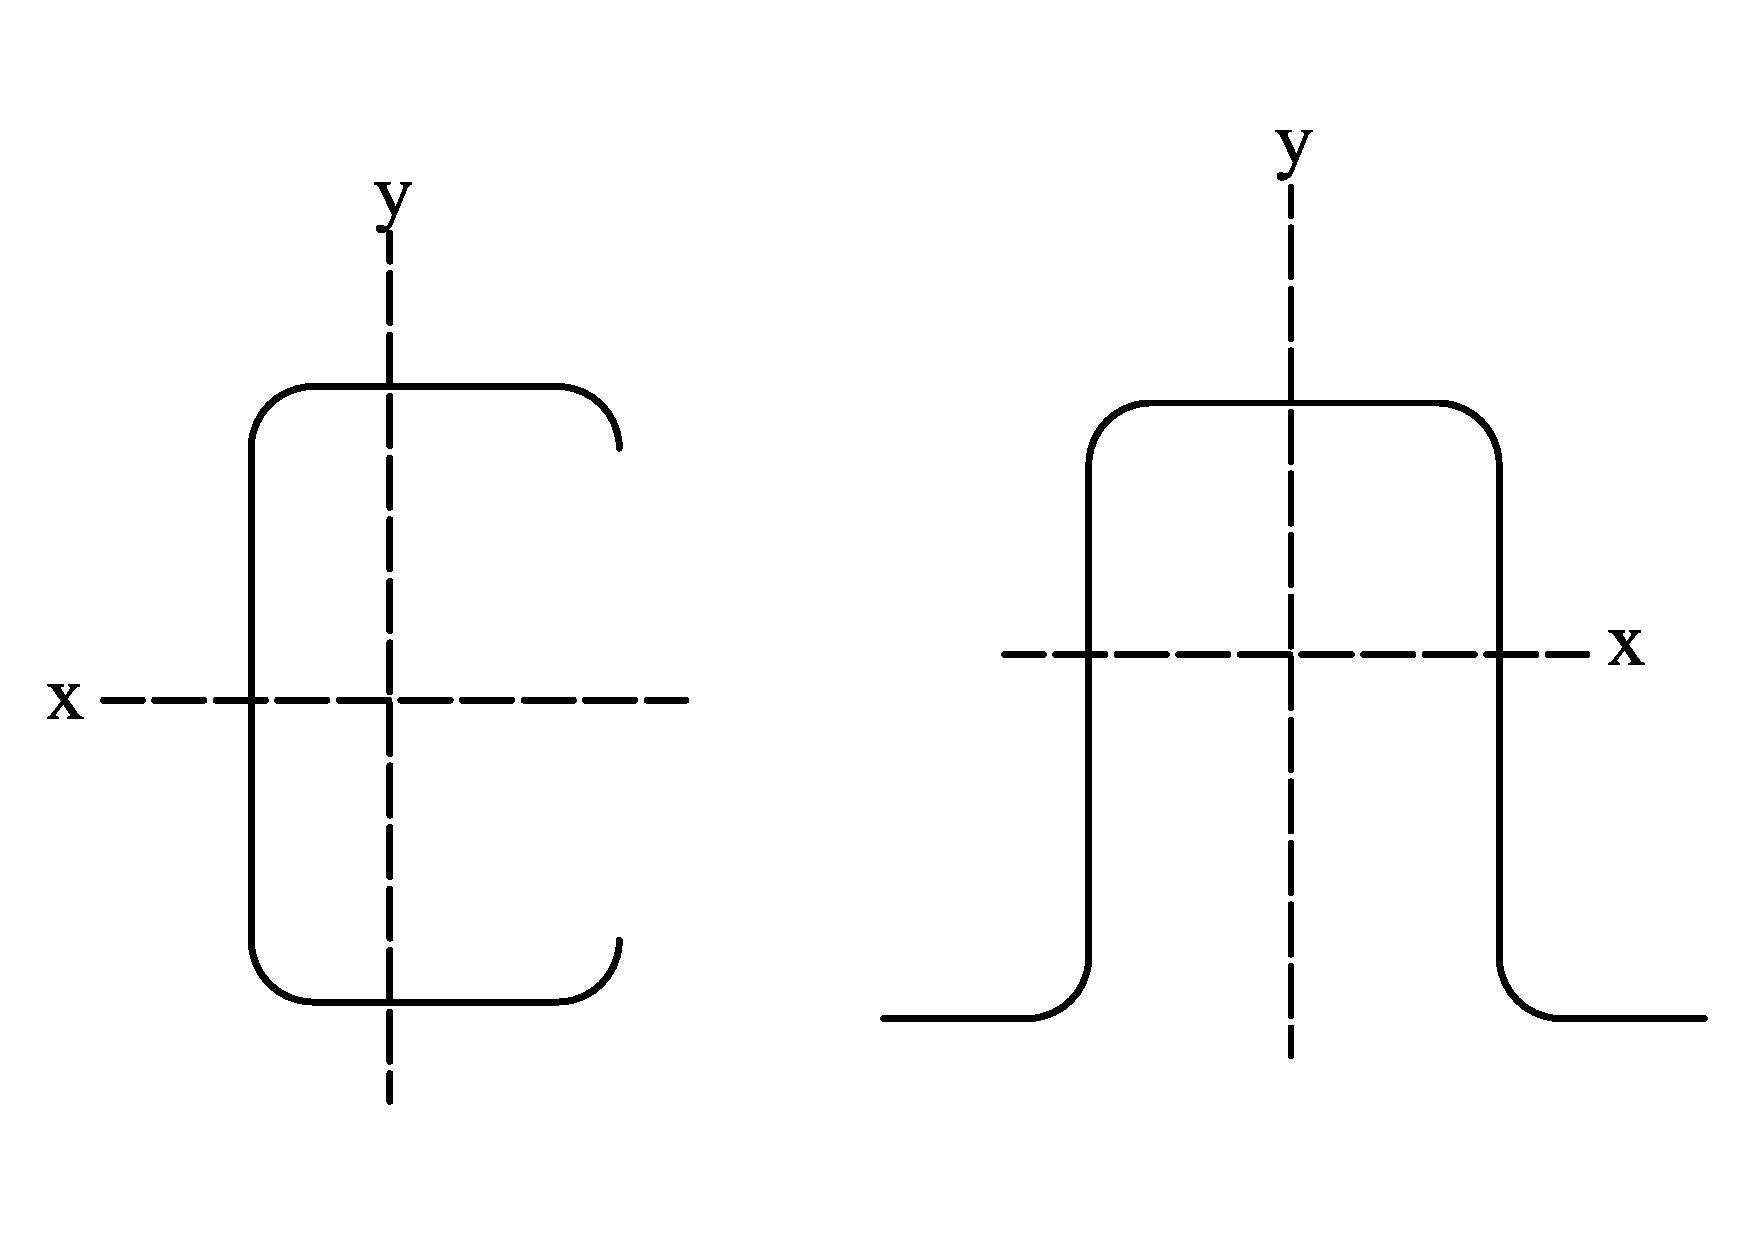
\includegraphics[scale=0.15]{singly_symmetric} & 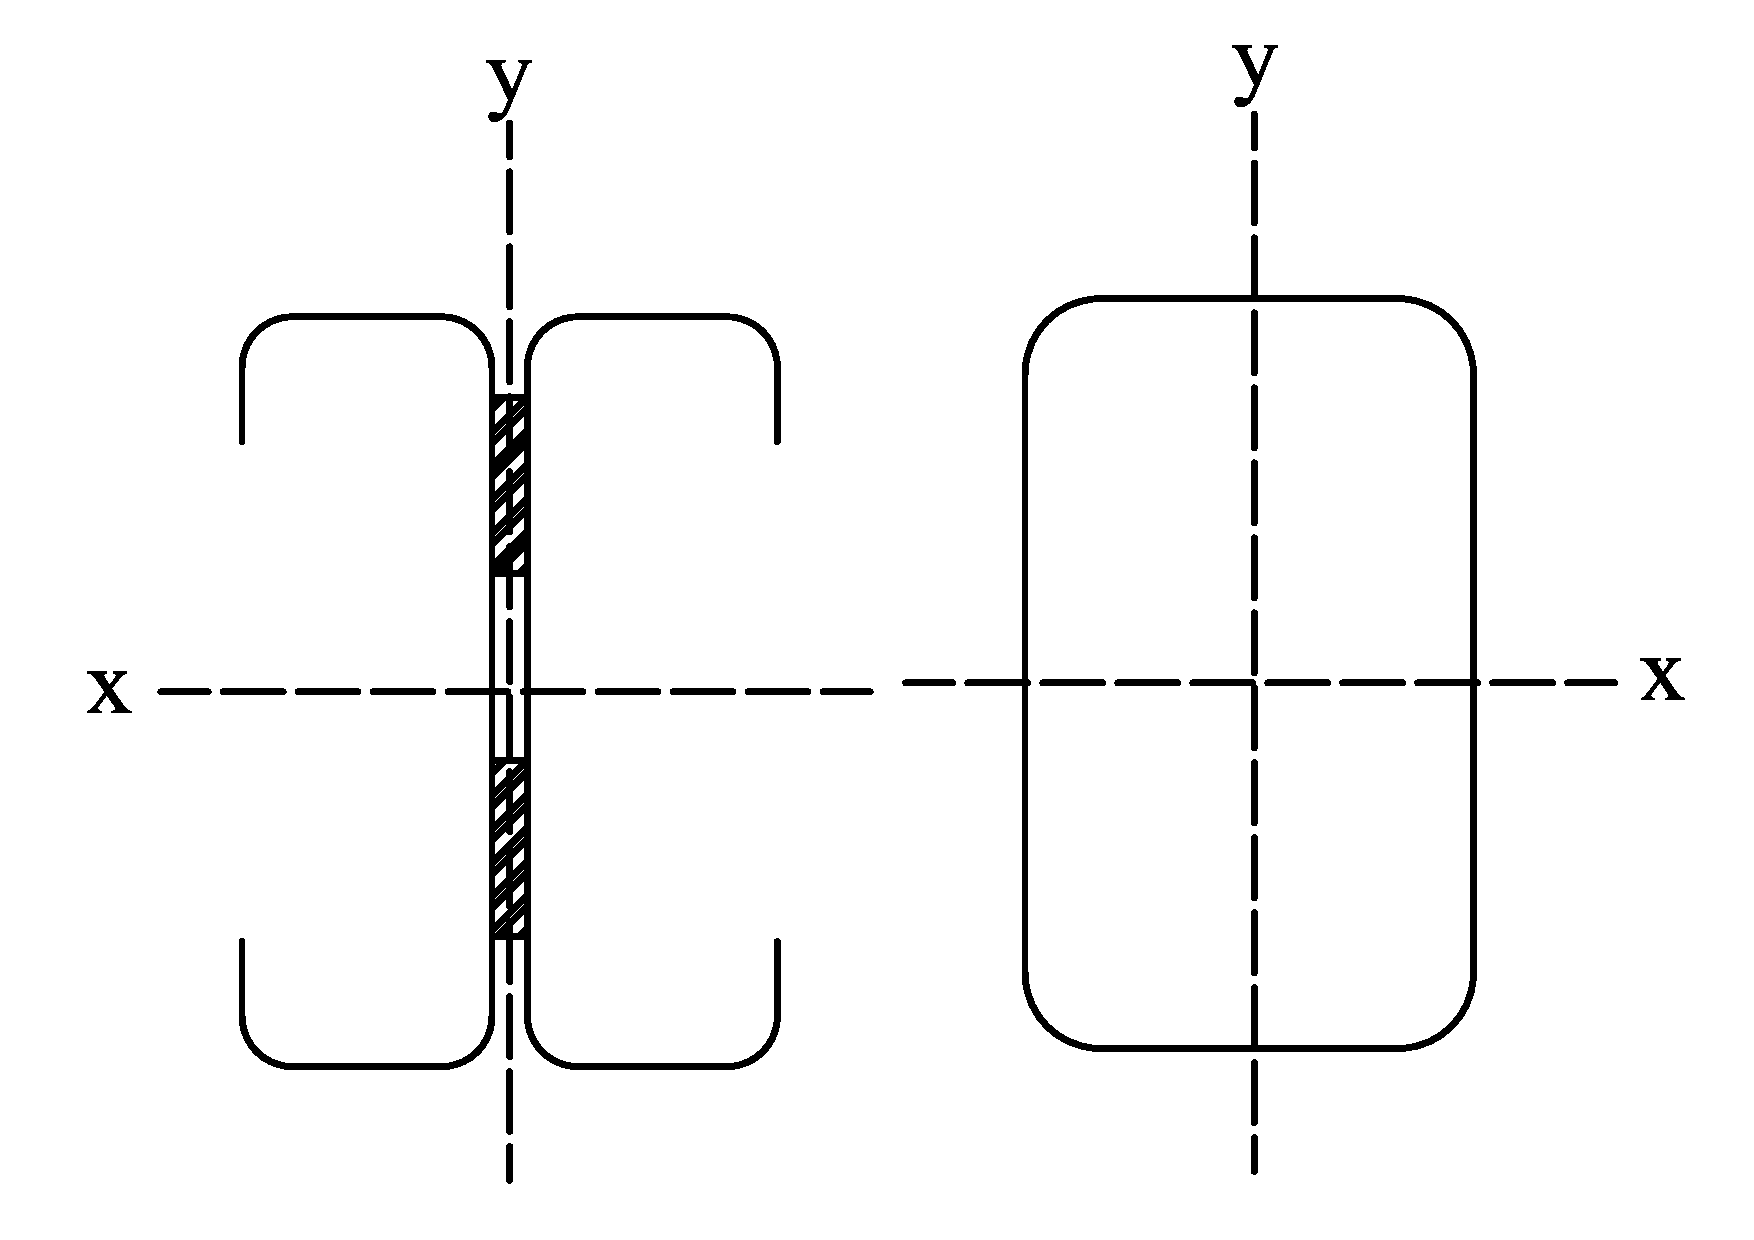
\includegraphics[scale=0.15]{doubly_symmetric} \\ 
			(a) & (b)  \\ 
			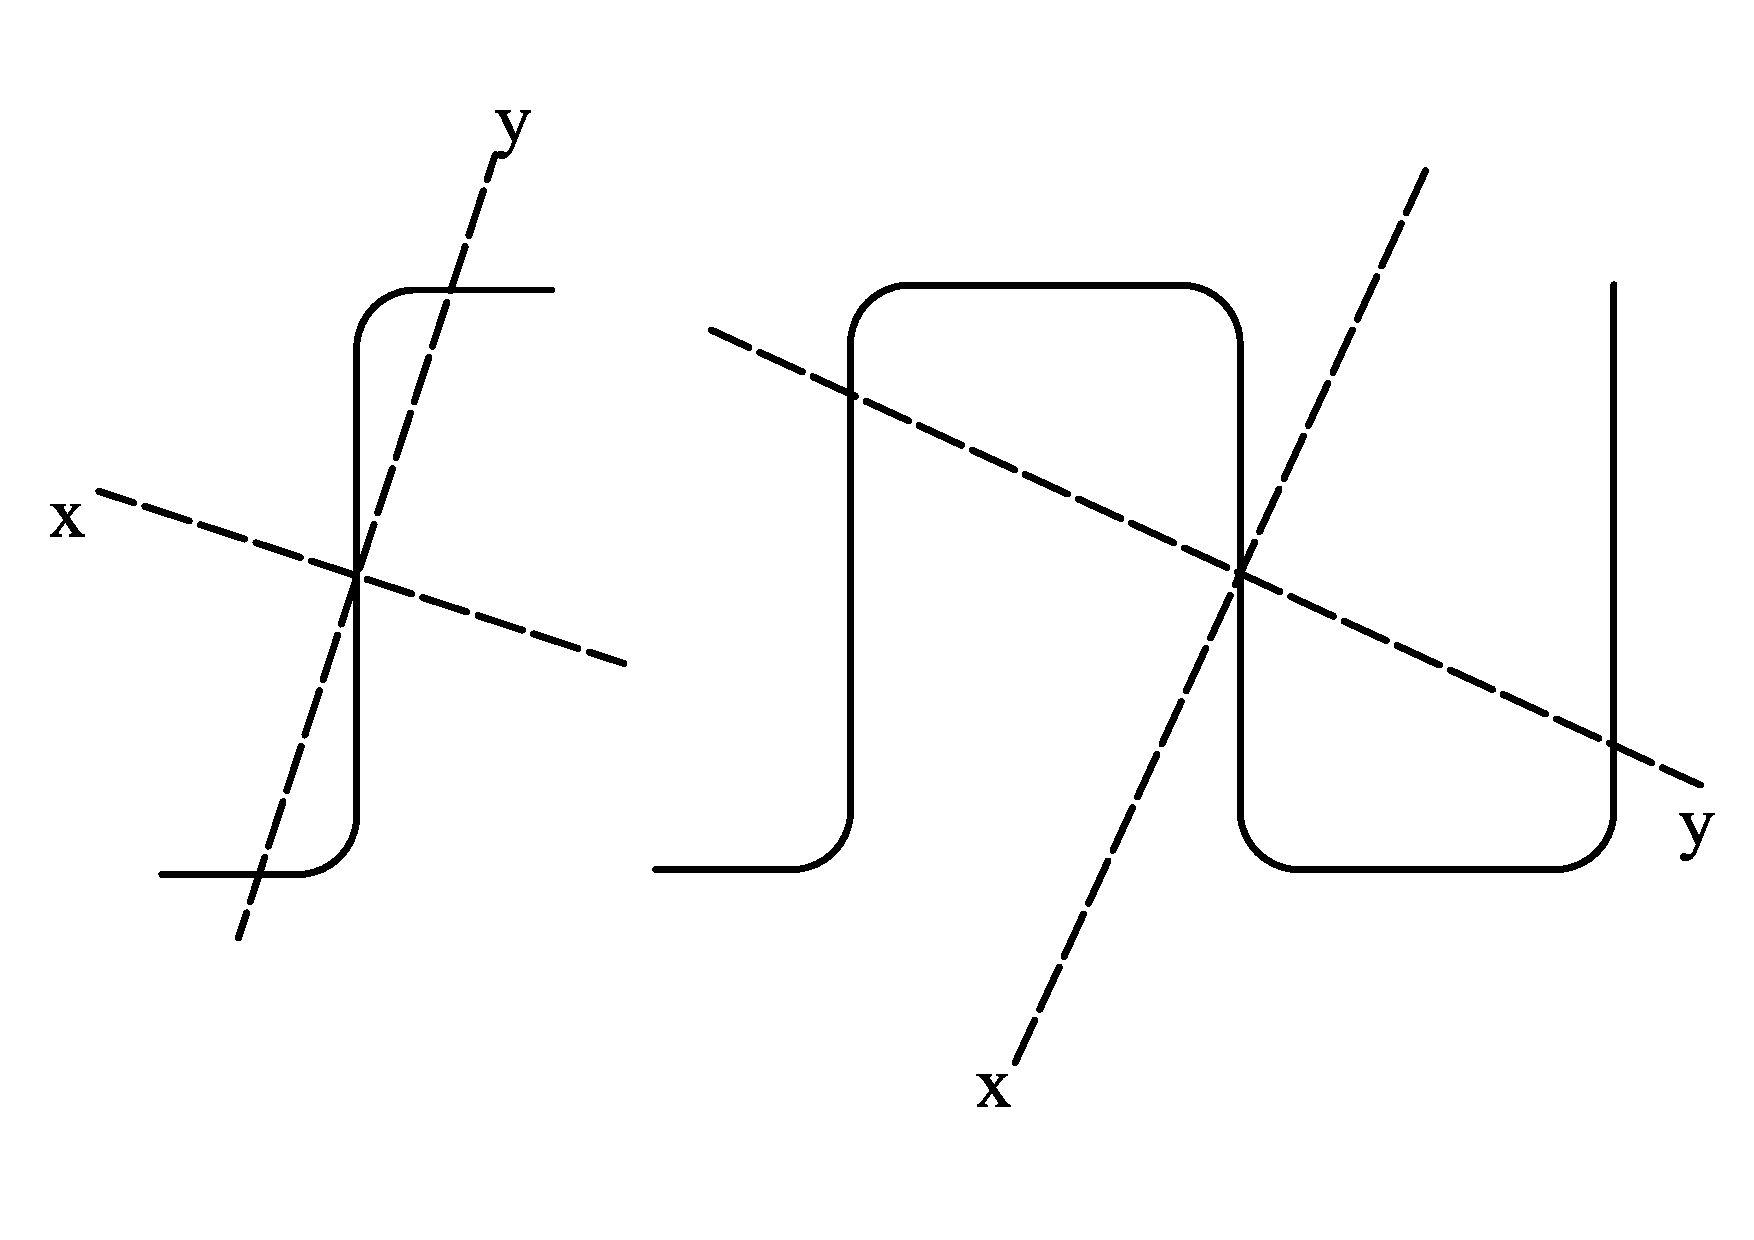
\includegraphics[scale=0.15]{point_symmetric} & 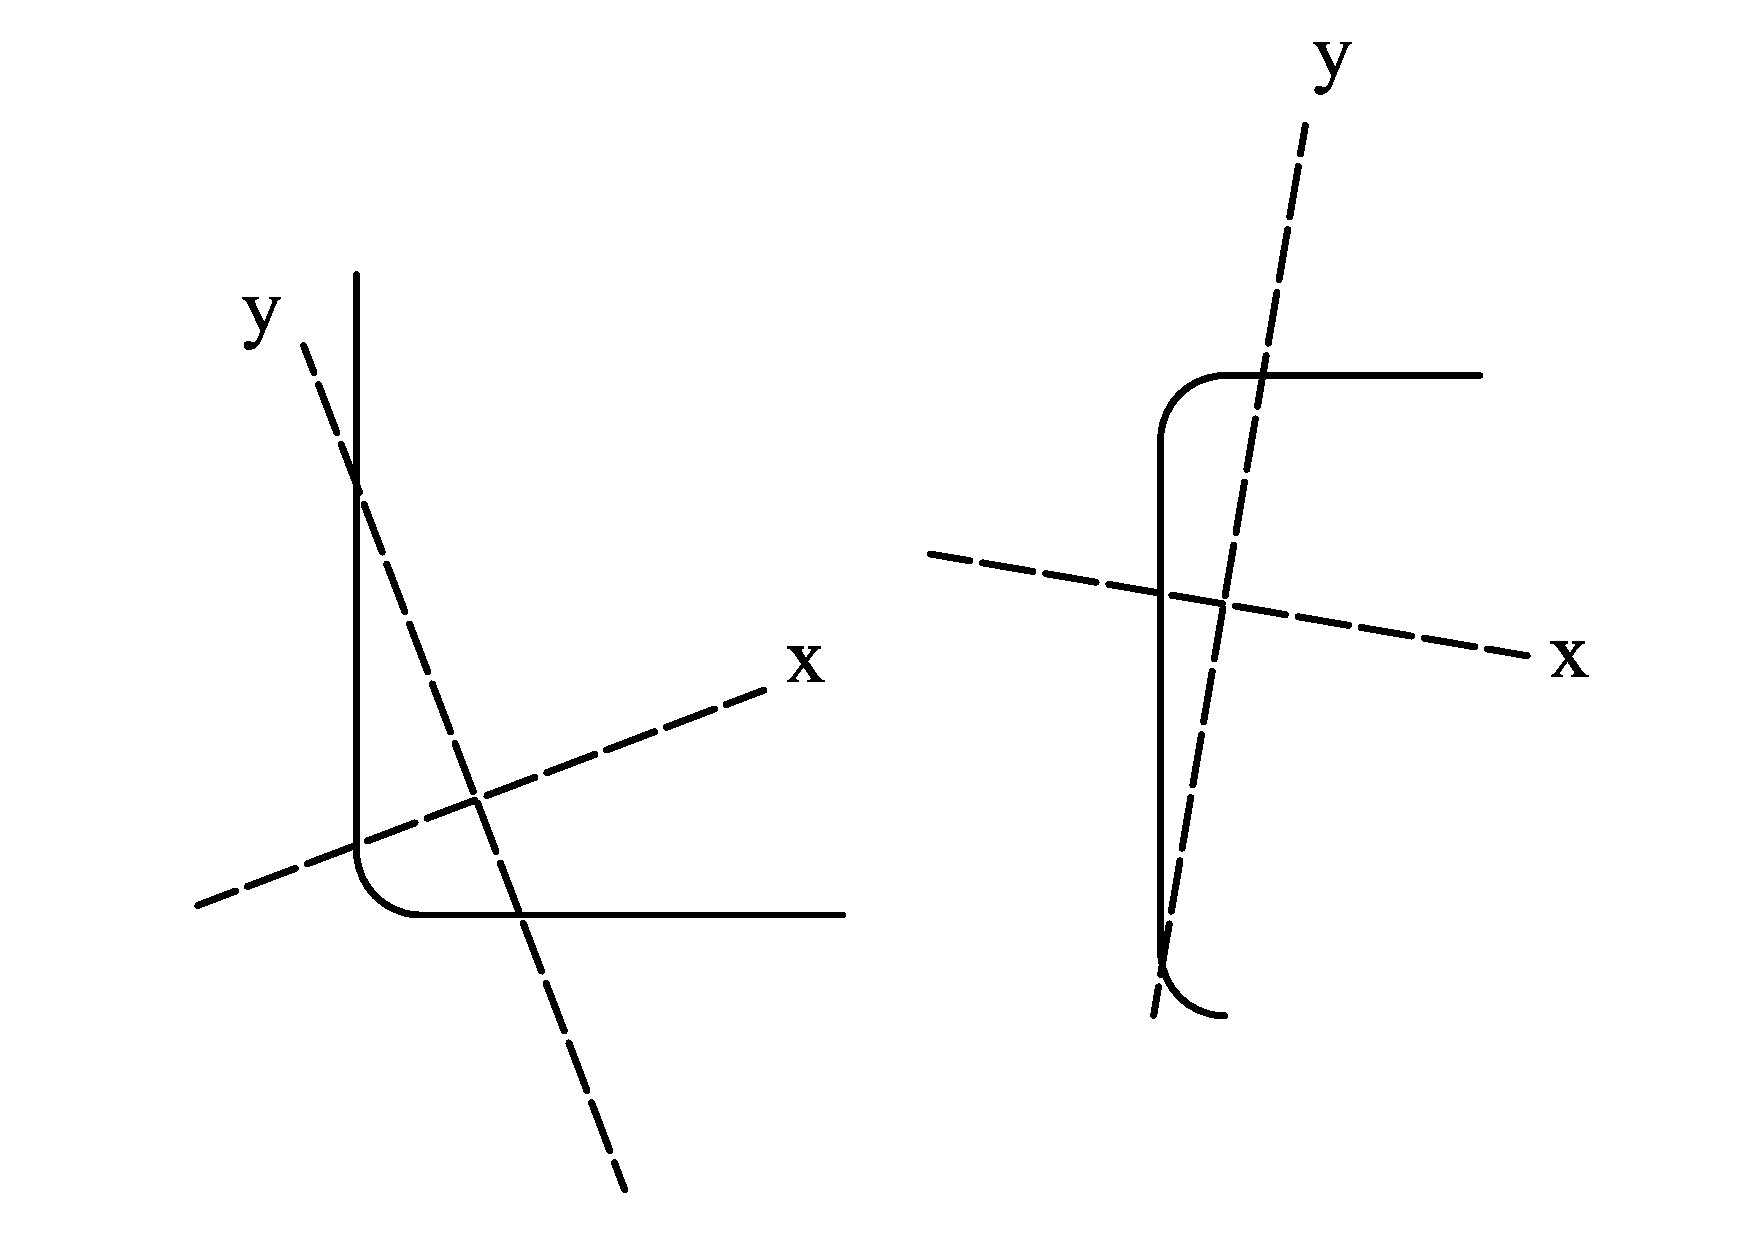
\includegraphics[scale=0.15]{non_symmetric} \\ 
			(c) & (d)  \\
		\end{tabular} 
		\caption{Different types of symmetric sections(a) Singly (b) Doubly (c) Point (d) Mono}
		\label{fig:symmetry}
\end{figure}
Hence, they are subjected to more complex buckling modes. When the mono-symmetric lipped channel studs are exposed to fire on one side, they are subjected to the following
\begin{itemize}
	\item Temperature gradient across the depth resulting in thermal bowing.
	\item Non-uniform mechanical properties across the cross-section as the hot flange mechanical properties are much less than those of cold flange.
\end{itemize}
\begin{figure}[htbp]
	\centering	
		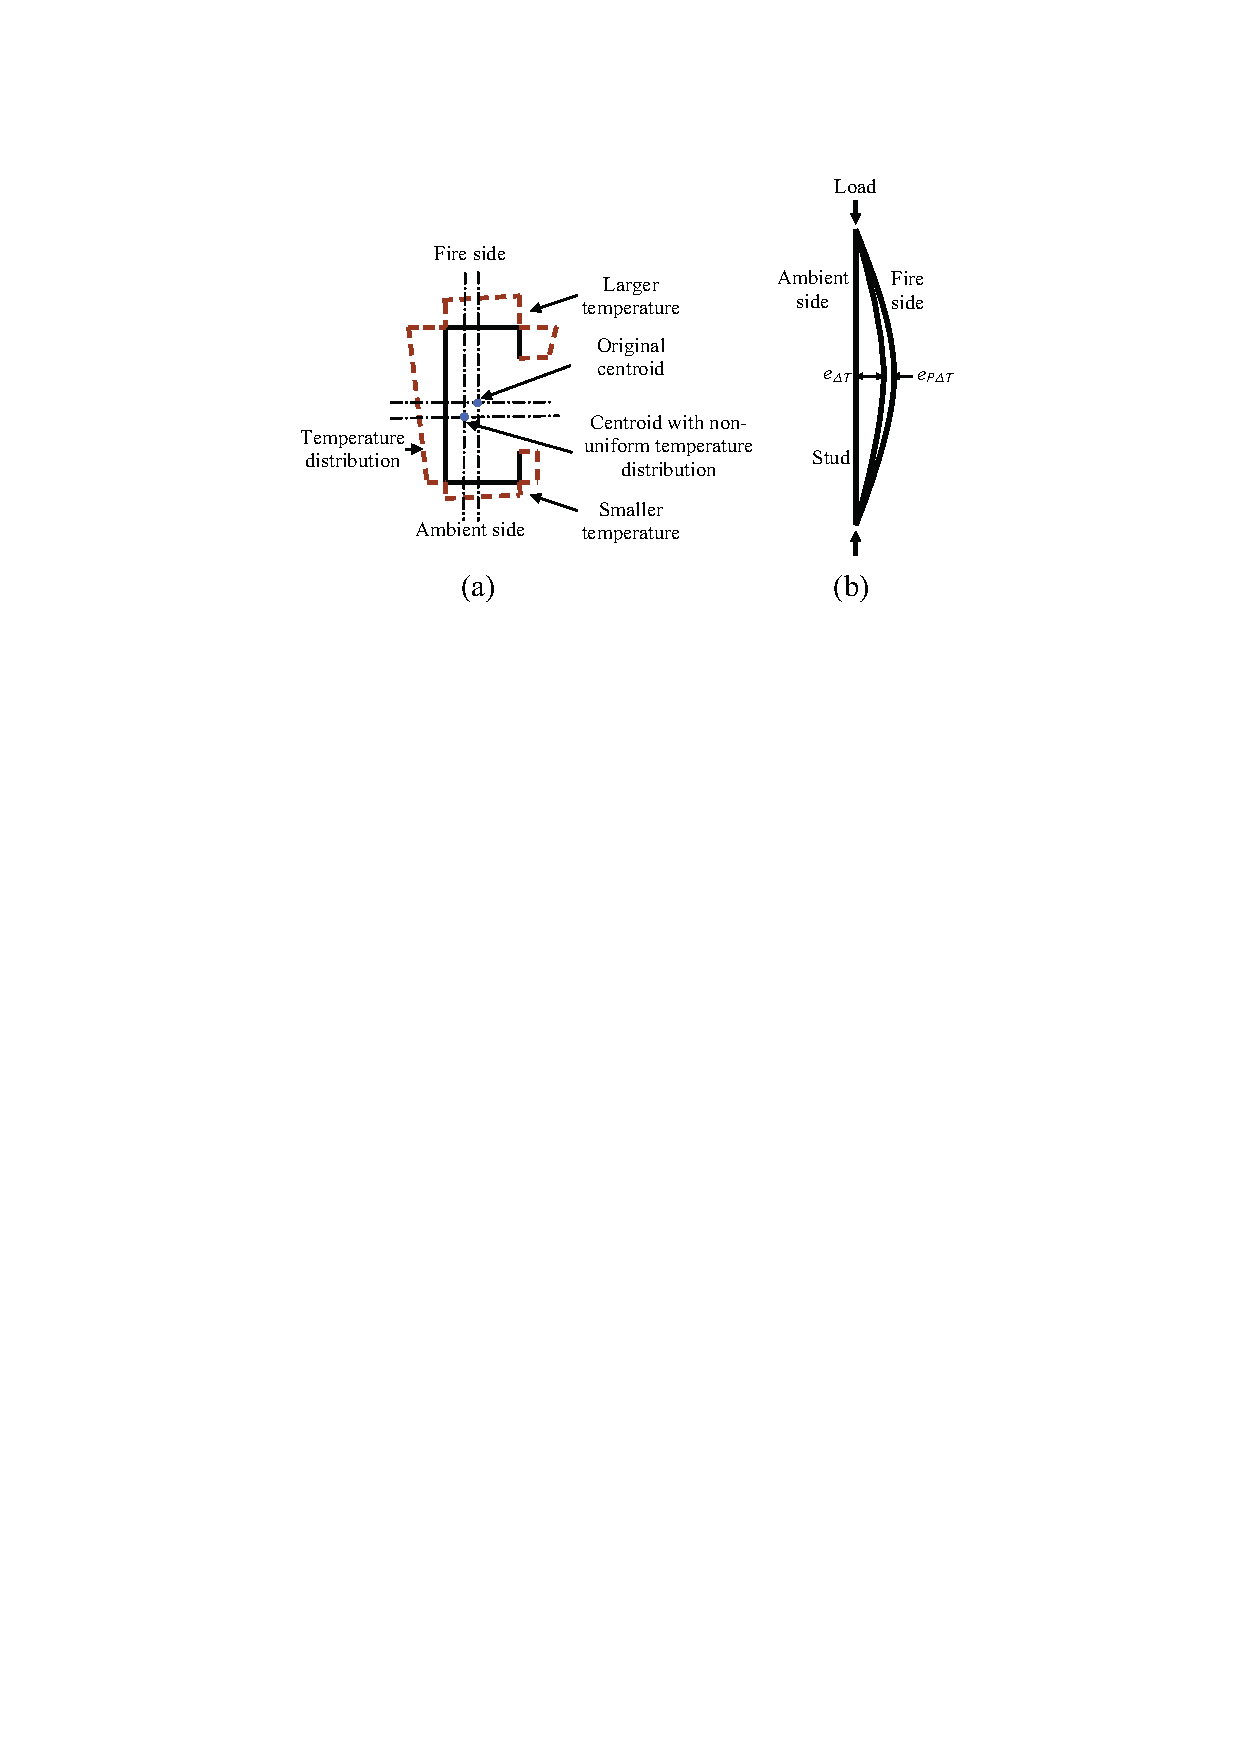
\includegraphics[width=8cm,height=5cm]{gunalan_nutemp}
		\caption{Neutral axis shift due to thermal bowing (\cite{Gunalan2014j})}
		\label{fig:gunalan_nutemp}
\end{figure}
\begin{figure}[htbp]
	\centering	
		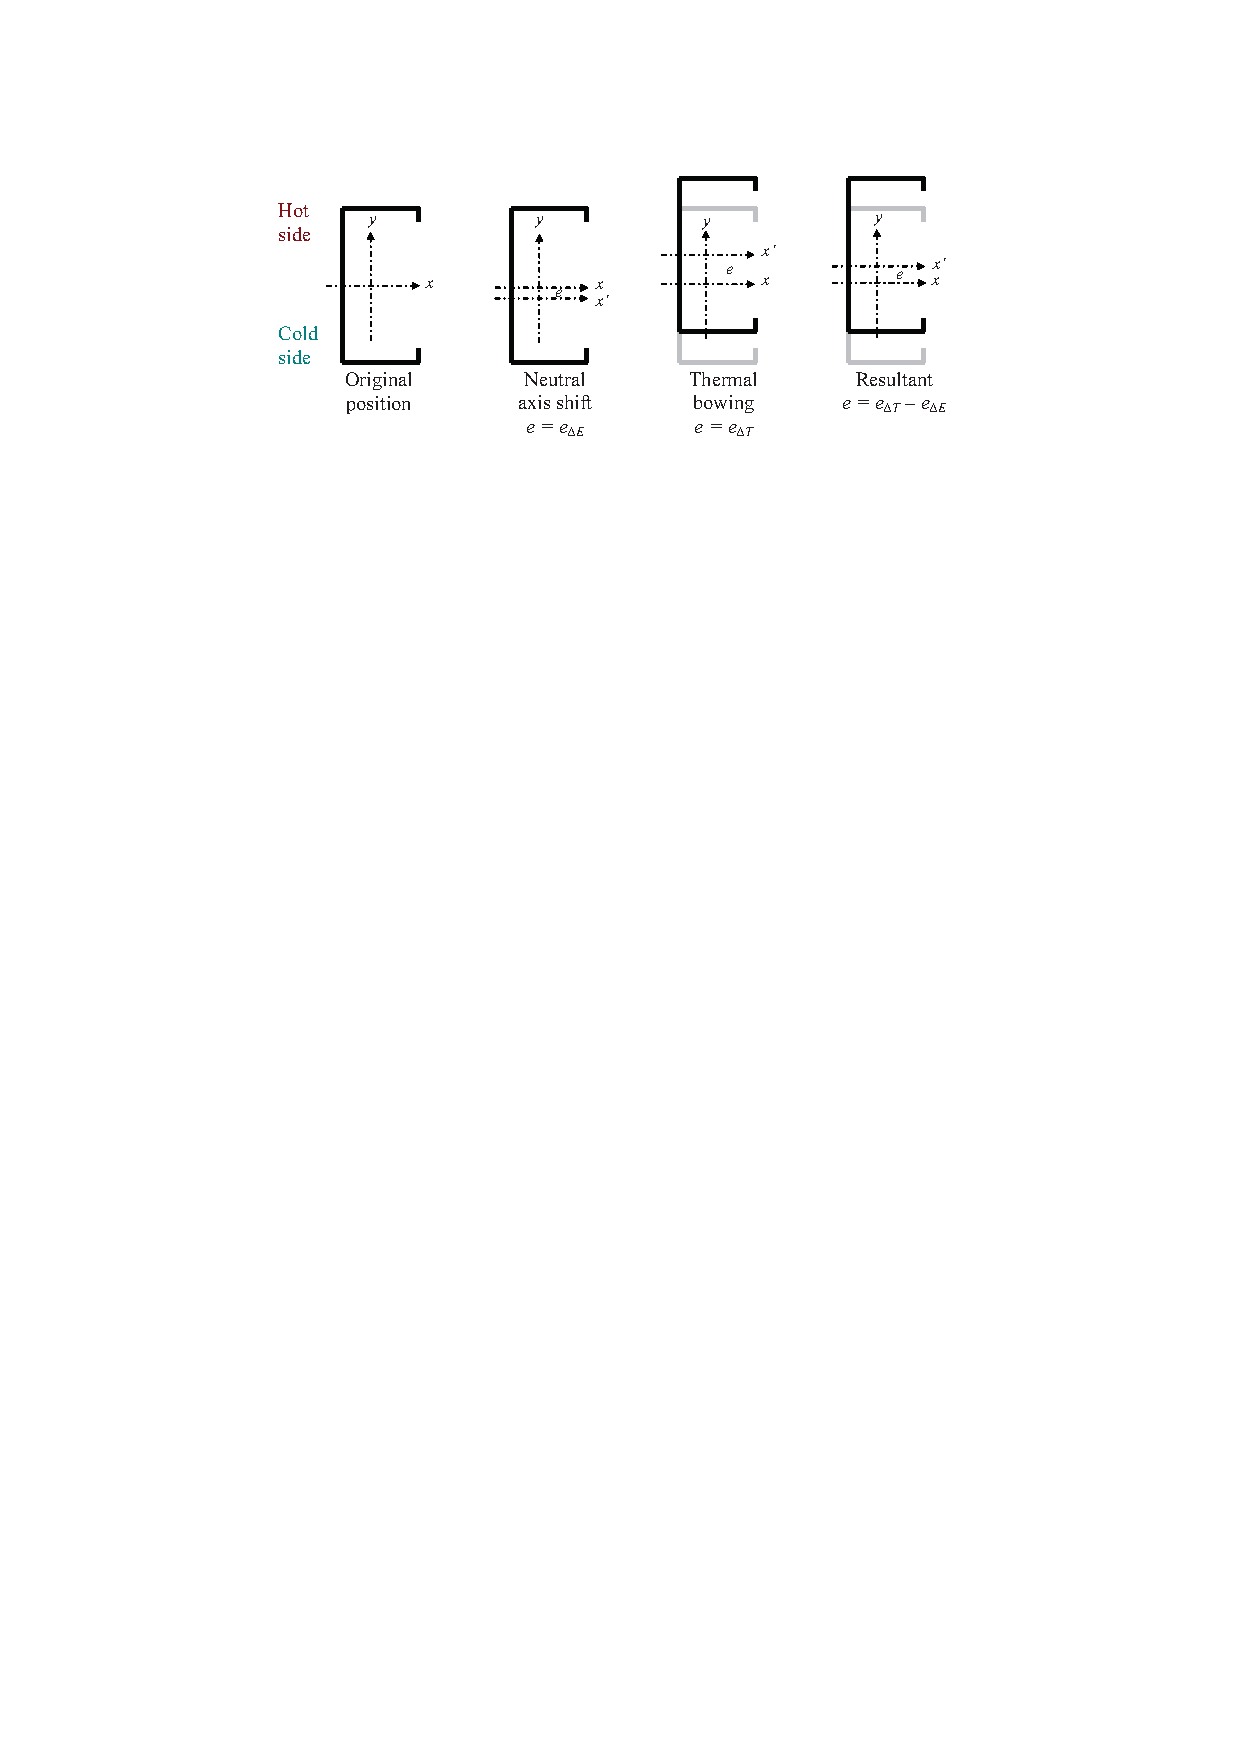
\includegraphics[width=8cm,height=4cm]{gunalan_nashift}
		\caption{Lateral deflection due to thermal bowing (\cite{Gunalan2014j})}
		\label{fig:gunalan_nashift}
\end{figure}
The presence of non-uniform mechanical properties leads to neutral axis shift of the stud section (\Cref{fig:gunalan_nutemp,fig:gunalan_nashift}). These actions caused by fire exposure on one side induce the thin-walled stud to be subjected to a bending moment in addition to the applied axial compression load.

\section{Complex LSF Wall Systems}
Complex LSF wall systems are needed and are being used in various applications in the building sector. Some of these wall systems are based on double and staggered stud configurations Figures \ref{fig:typical-complex}~(a) to (c). To withstand heavy structural loads in the case of mid-rise construction, such systems are preferred. Also, to achieve higher acoustic insulation in places where sound insulation is important, these wall systems are used. Double stud walls are those with two parallel rows of studs with studs located directly opposite to each other whereas studs in parallel rows are staggered in case of staggered stud walls. Lipped channel steel sections are widely used as the studs in LSF walls. The major components of the double and staggered stud walls include two rows of cold-formed steel studs, tracks, noggings, bracings, and plasterboards. These components are fixed together using self-piercing screws of different types. The physical and thermal properties of the double and staggered stud wall components are similar to single stud LSF walls. But due to the increased cavity depth, the behaviour of the components such as studs under fire exposure is different. The acoustic, thermal and structural performance of double and staggered stud walls is likely to be superior compared to single stud walls. Plasterboard manufacturers such as USG Boral, CSR and Knauf Plasterboard include double and staggered stud wall systems in their product manuals although their main focus is on double stud wall systems. To date no detailed research has been undertaken on the thermal and structural behaviour of these complex wall systems with different configurations. 
\begin{figure}[!htbp]
	\centering
		\begin{tabular}{c}
			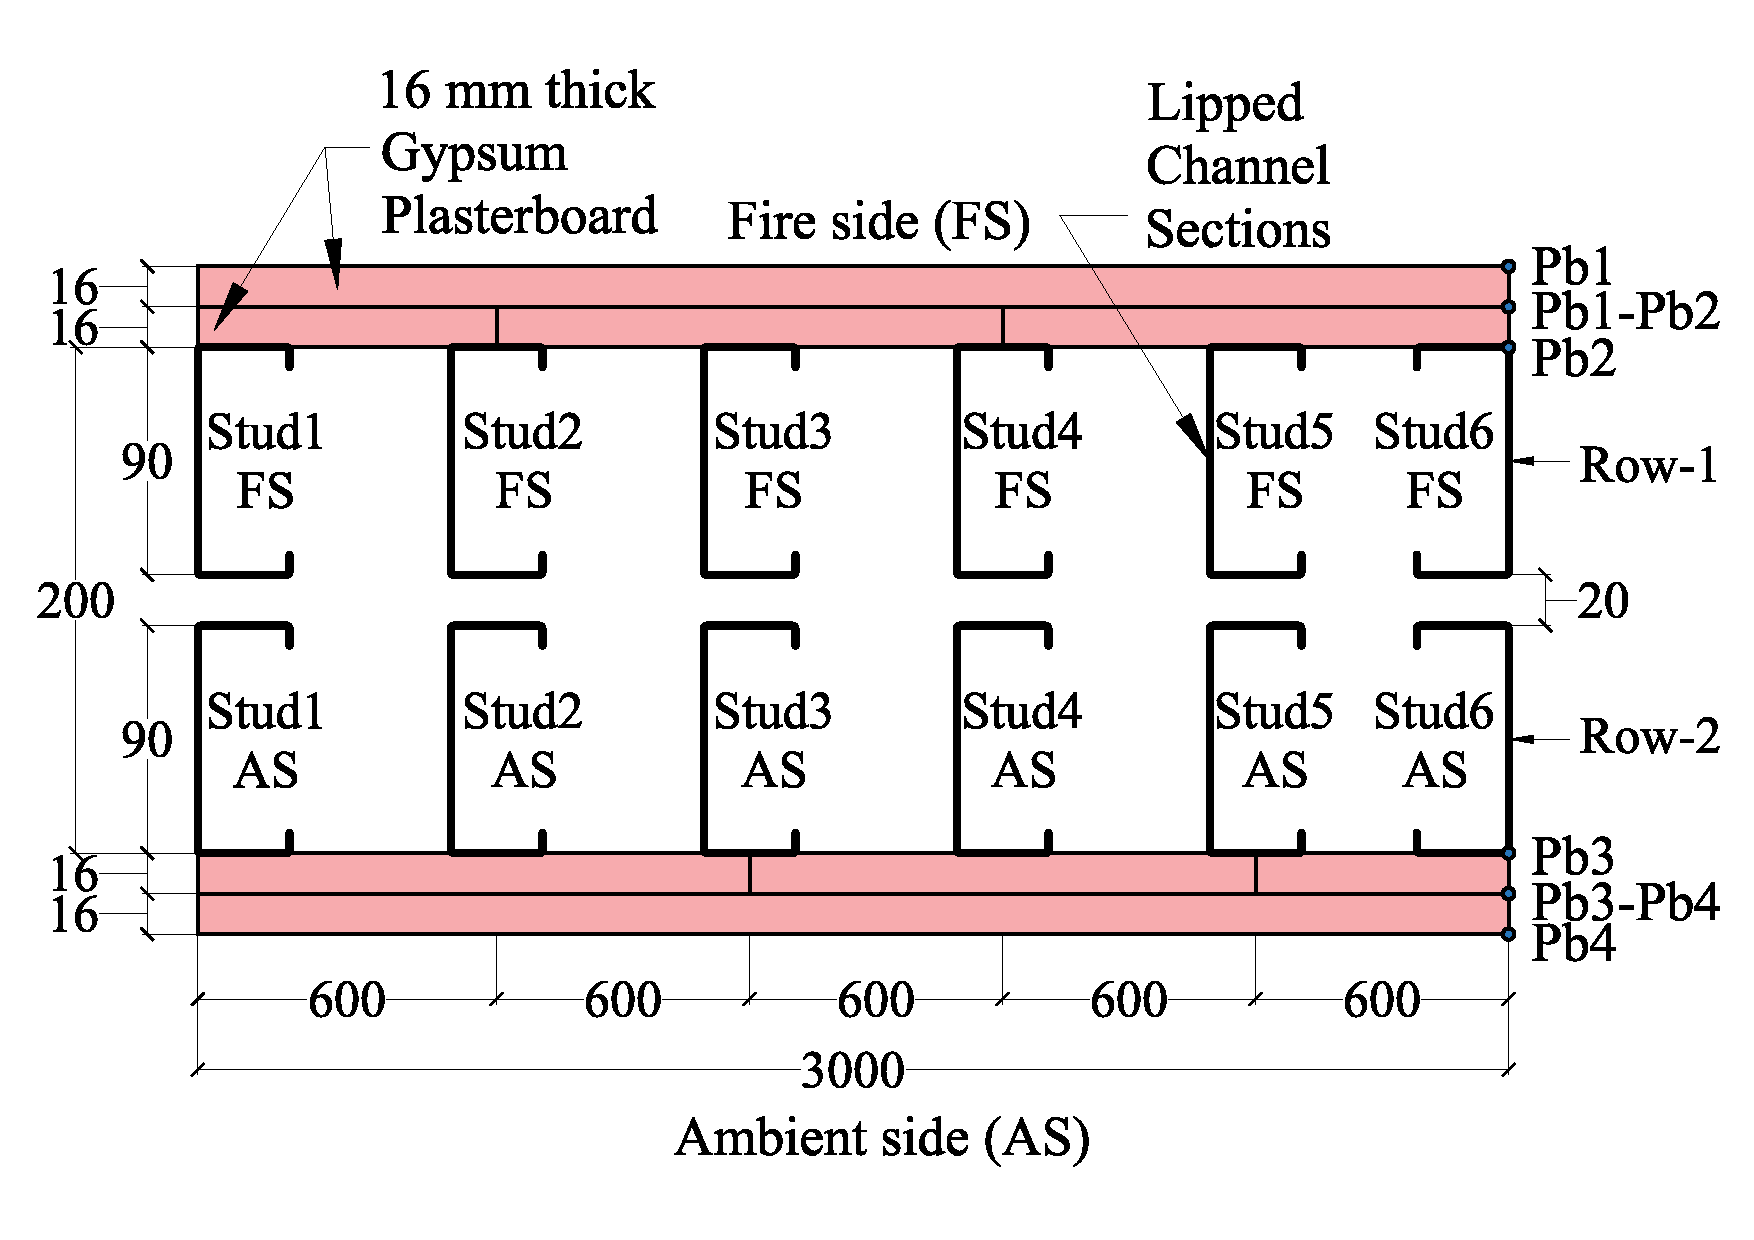
\includegraphics[width=8cm, height=5cm]{T1-plan} \\
			(a) \\
			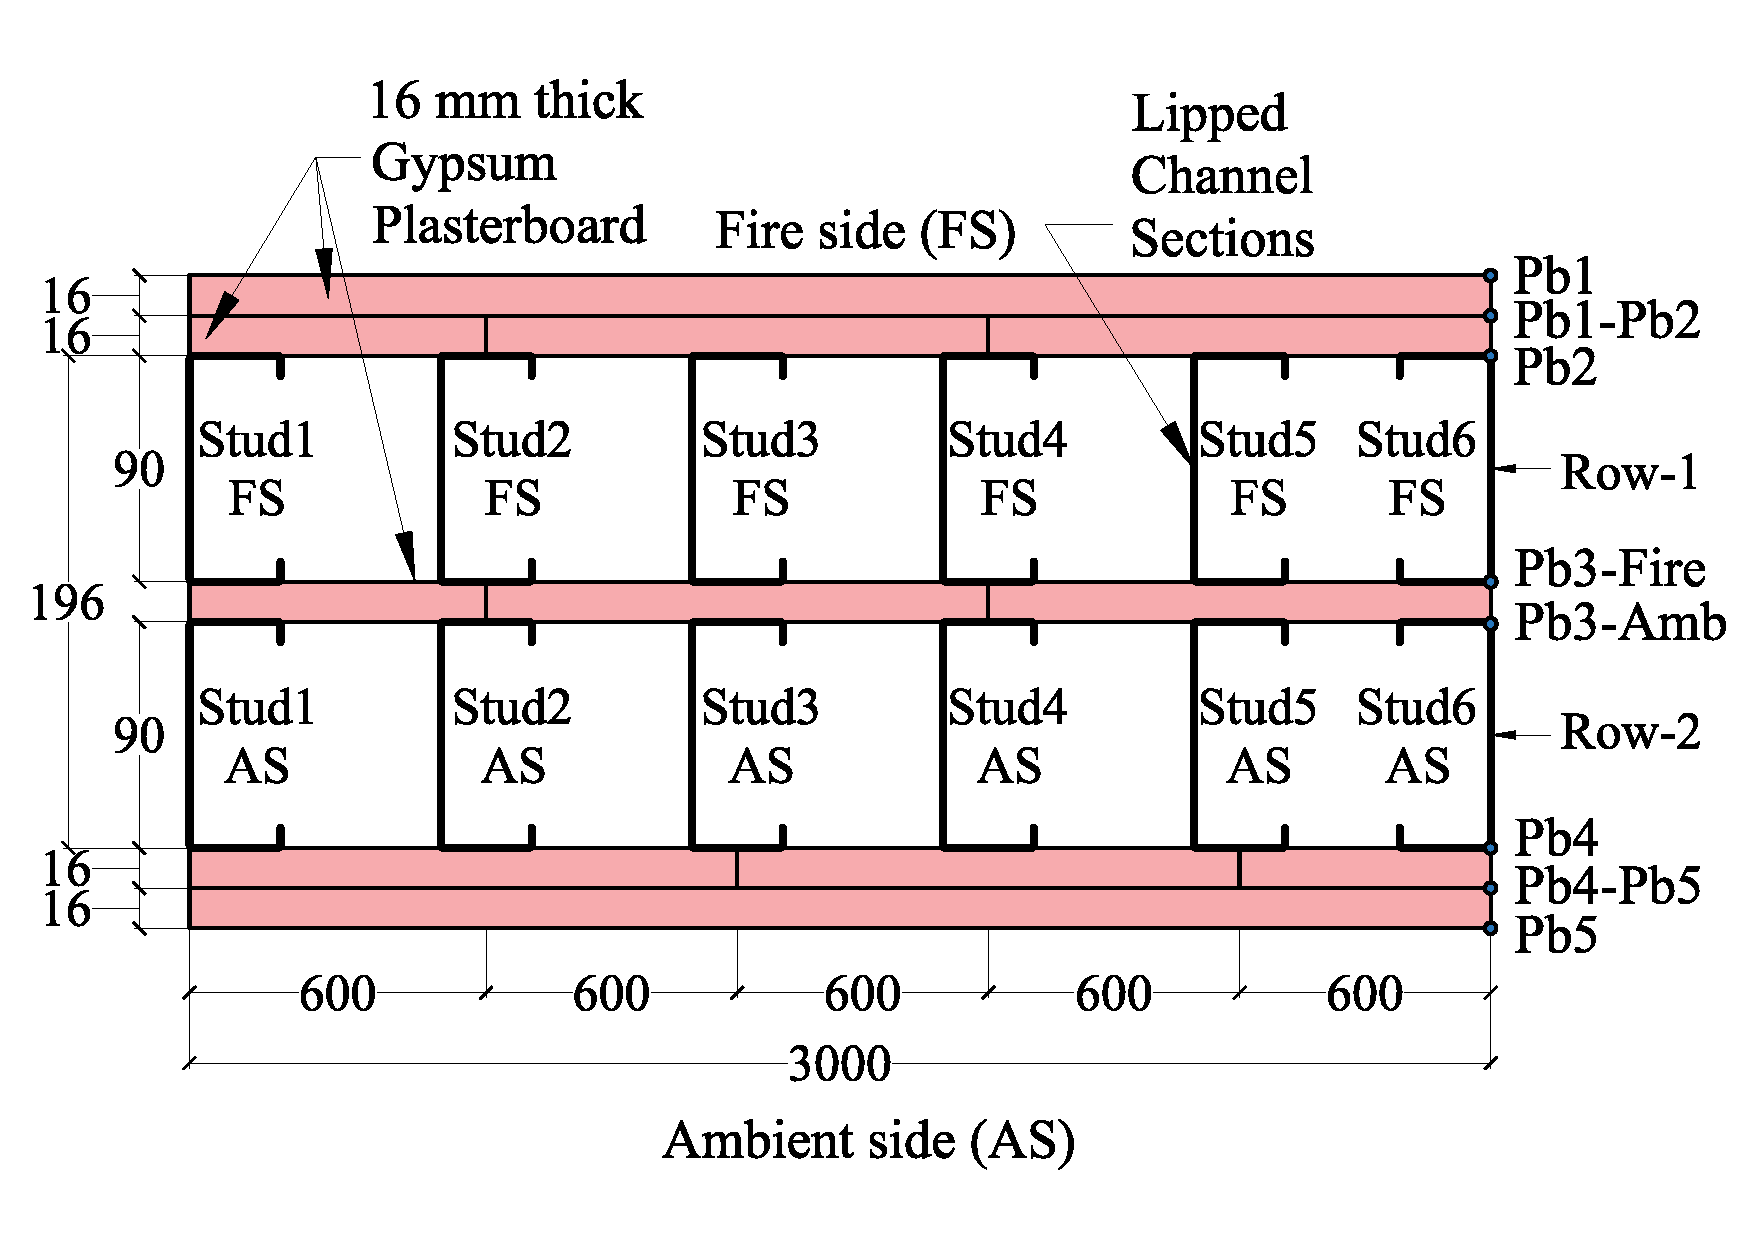
\includegraphics[width=8cm, height=5cm]{T8-plan} \\ 
			(b)  \\ 
			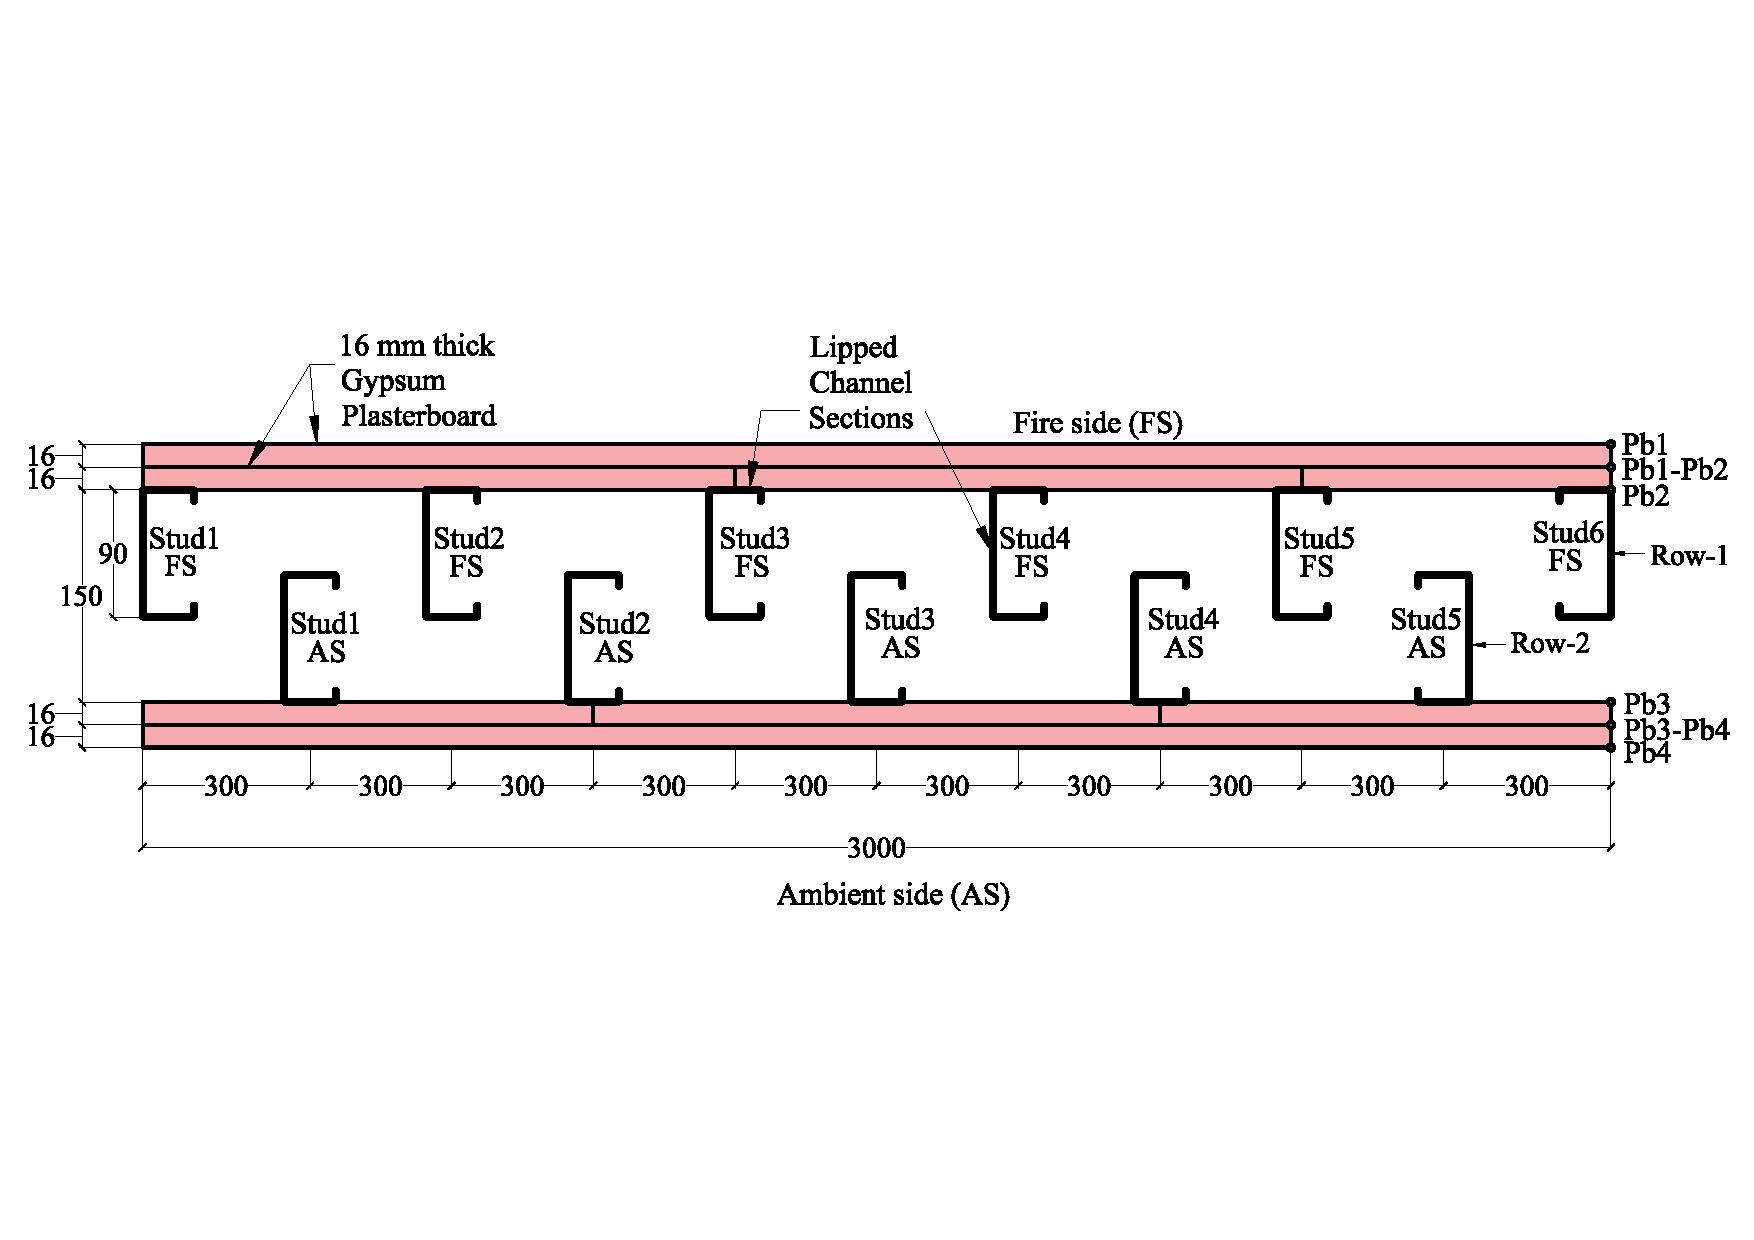
\includegraphics[scale=0.45]{T9-plan} \\ 
			(c)  \\ 
		\end{tabular} 
		\caption{Typical complex LSF wall configuration (a) Double stud (b) Shaftliner (c) Staggered stud }
		\label{fig:typical-complex}
\end{figure}

The construction of double stud LSF walls is also different from that of single stud walls. The double stud walls generally consist of a small air gap as shown in \Cref{fig:typical-complex}~(a) or may contain a shaft liner or a plasterboard layer between the stud arrangement as shown in \Cref{fig:typical-complex}~(b). These arrangements are present to split the cavity into two or more to yield a better fire and acoustic performance. The presence of two rows of studs in different arrangements within the LSF wall will increase the load carrying capacity of the wall system and its fire performance. This will be beneficial in mid-rise buildings as the loads on the walls will be higher when compared to low rise buildings.

\section{Research Problem}

Increasing the Fire Resistance Level (FRL) of LSF wall is the need of the day. Researchers implement their ideas to ultimately increase the FRL of wall systems and make it structurally stable so that in the event of fire outbreak loss of life due to structural failure can be nullified. Past research studies focused only on varying the plasterboards by changing the type of boards, increasing the number of plasterboard layers in the wall, changing the type of stud section, improving the thermal performance of plasterboard using an external insulation layer etc. to achieve higher FRL. Effects of the arrangement of studs inside the wall via more complex wall systems was not the primary focus in many research studies. Earlier investigations focused on walls with less than 3 m height, which are primarily used in residential buildings. In residential buildings, the acoustic insulation is not a major concern as the intensity of sound for transmission through the wall is minimum. But in movie theatres, studios and in wall partitions between houses in an apartment, acoustic insulation is very important and the wall height can exceed 3 m. Especially in situations where the wall height exceeds 3 m, single stud arrangement cannot be used as the cold-formed steel sections are slender in nature. In these situations, complex wall systems with double rows of studs with or without a middle layer of plasterboard or shaftliner can be used. They can also be used as staggered stud wall systems (\Cref{fig:typical-complex}). Similarly, with the focus on developing mid-rise building systems using cold-formed steel members, LSF wall systems with complex wall systems are needed in the lower storeys for higher load bearing purposes. In mid-rise buildings, the axial compression load acting on the bottom stories will be higher when compared with the top levels. Fire resistance and structural adequacy of building components in mid-rise buildings are utmost importance to prevent a structural collapse during fire outbreak. However, past research has addressed only the thermal and structural behaviour of LSF wall systems with single row of studs. This research will therefore focus on the complex LSF wall systems with double and staggered stud LSF wall systems. 

Another important research problem is the lack of a robust numerical model and analysis technique for LSF walls exposed to fire conditions. Many parameters such as free water evaporation from the plasterboard, effects of cavity radiation due to heat transfer from one face of the wall to another, pressure build-up within the cavity due to heat transfer and air movement within the cavity through natural convection were not considered in the past numerical modelling studies to reduce the complexity of numerical analysis. 

Fire tests of load bearing and non-load bearing walls are an effective means to investigate the thermal and structural performance of complex LSF wall systems. But when the cost and time consumed in these tests are taken into consideration, it becomes uneconomical and practically impossible to study many iterations of wall systems within a short span of time. With the advancement of high-performance computing in recent times, it becomes beneficial for the researchers to study the thermal and structural behaviour of LSF walls with ease. Finite element analysis (FEA) is considered as the key to many multi-physics problems. Research on the thermal and structural performance of LSF wall systems is carried out using FEA software such as ABAQUS, ANSYS etc. Most common heat transfer problems such as combustion inside an engine is modelled and analysed by Computational Fluid Dynamics (CFD) technique as heat transfer happens in 3-dimensionsional space. Past research has focused on modelling the design or real fire as 1-dimensional entity only. Therefore, attempts should be made to use CFD models to investigate the thermal behaviour of complex LSF wall systems by considering the fire loads in 3-dimensional space.

\section{Research Aim}

The aim of this research is to investigate the thermal and structural performance of selected complex double and staggered stud LSF wall systems using full scale standard fire tests and advanced numerical modelling. The key tasks of this research to achieve this aim are as follows. 
\begin{itemize}
	\item Undertake a detailed review of complex LSF wall systems and their fire performance, and thermal and mechanical properties of wall components and, establish their appropriateness.
	\item Conduct a series of full scale standard fire tests of double and staggered stud wall systems to investigate their thermal and structural performance in fire. 
	\item Compare the full-scale fire test results with the available fire test results of conventional single stud wall systems to evaluate the effects of complex stud arrangements on structural and thermal performance.  
	\item Develop advanced finite element models to simulate the thermal and structural performance of double and staggered stud wall systems exposed to fire conditions and validate them using full scale fire test results.
	\item Improve the fundamental understanding of the thermal and structural performance of double and staggered stud wall systems through the use of validated finite element models in investigating the LSF wall behaviour and failure modes of studs in detail.
	\item Undertake a detailed parametric study of double and staggered stud wall systems with different structural and thermal parameters of LSF wall components. 
	\item Investigate the suitability of existing fire design rules in the Australian and European fire design standards for complex LSF wall systems and if needed, develop improved fire design rules and simple design methods to predict the fire resistance levels and axial compression capacities of cold-formed steel studs in complex LSF wall systems exposed to fire.
\end{itemize}

\section{Outline of Thesis}

Based on the research aim and the specific tasks as listed above, this research was conducted in a sequential manner and a brief outline of the contents included within the chapters are presented next.

\textbf{\Cref{ch:Literature}} details the extensive literature review conducted on LSF walls. Topics include the ambient and fire performance of simple and complex LSF wall assemblies. This covers the experimental and numerical investigations on LSF walls. Initial investigations were carried out by sampling the real-time problems faced by the LSF wall industry with respect to complex wall systems (double and staggered stud walls). Literatures were collected and reviewed to identify the problems to be taken up for the current research. Ground surveys by contacting industry experts to know about the current practice in the complex LSF wall arrangements such as double and staggered stud walls were carried out to determine the best possible complex LSF wall configurations to be investigated in the current study. Finally, a summary of the reviewed literature was made and the possible techniques to address the research aim are proposed.

\textbf{\Cref{ch:Ambient}} presents the ambient temperature capacity test results conducted on selected complex LSF walls based on the detailed literature review. Test results include the axial compression capacity, axial displacement and lateral deflection curves. The buckling behaviour of studs in double and staggered LSF wall configurations under axial compression is also discussed in detail. Numerical investigations through finite element analyses conducted on double and staggered LSF wall configurations to predict the ambient axial compression capacity are also discussed. 

\textbf{\Cref{ch:Fire}} reports the findings of one small scale fire test and 10 full-scale fire tests conducted on double and staggered LSF wall systems. Illustrations are made for the tested complex LSF wall configurations and fire test results in the form of time-temperature curves are presented in detail. Increase in the FRL of the complex LSF walls was noticeable in comparison with similar single stud LSF wall assemblies. The detrimental effect of cavity insulation in complex LSF walls was also investigated. Detailed comparison of the fire test results are made against full-scale fire test results of single stud LSF walls and the unique heat transfer mechanism in complex LSF walls are summarised. 

\textbf{\Cref{ch:FE-Thermal}} presents the developed FE thermal models to predict the thermal performance of complex LSF wall systems. Firstly, three different software packages were used to develop thermal models and a detail comparison was made amongst them to find the most appropriate software package to use for developing the thermal models. A detailed comparison was made considering the advantages and shortcoming in the thermal model results and the numerical model results were validated against the conducted small-scale and full-scale experimental results to establish the suitability of the model. Based on the developed model, a detailed parametric study was conducted on complex LSF wall configurations to predict the fire performance and the corresponding results were also discussed in detail.

\textbf{\Cref{ch:FE-Structural}} details the FRL predictions from structural model which was developed alongside the thermal models to predict the structural behaviour of the studs in fire. The structural model inputs were extracted from the fire test results from \Cref{ch:Fire,ch:FE-Thermal} and the FRL predictions were made. Non-cavity insulated LSF walls were found to result in better FRL in comparison with cavity insulated LSF walls. The FRL predictions were made based on different load ratios based on the axial compression capacity determined in \Cref{ch:Ambient}.

\textbf{\Cref{ch:FE-Parametric}} presents the parametric analysis results conducted from FE thermal and structural models. The parameters for the stud includes different wall configurations and stud thicknesses. FRLs of the selected wall configurations are presented in table and the closest FRL in min corresponding to the BCC is also provided. 

% \textbf{\Cref{ch:Design}} covers the DSM based failure time predictions for complex LSF wall configurations under different load ratios. The suitability of the existing equations used for single stud LSF walls in predicting the failure times for complex LSF walls was investigated and summarised. The suitability of the existing design equations in comparison with the numerical models is also discussed.

\textbf{\Cref{ch:Conclusions}} provides a summary of the findings from this research study. Conclusions are drawn from the experimental and numerical investigations and suitable recommendations are also proposed for future work in relation to the fire performance of complex LSF walls.

